\documentclass{masterthesis_ceng}
% masterthesis for Computer Science
% masterthesis_ceng for Computer Engineering
% use the [nocoverpage] option to speed up compilation by skipping the cover page

% the configuration is in the preamble.tex file, read it and modify it to change
% the document appearance and included packages
\input{preamble}

% by default, we use the biblatex package to manage the bibliography
% if you prefer to use bibtex, comment the following line and uncomment the
% relevant lines at the end of the document
\addbibresource{bib.bib}

\input{acronyms}

\begin{document}

\title{ Flatness Filtering for Honeyword Generation }
\author{Sona Hosseinzadeh Mahdavi} 
 

% important for when you'll submit your thesis: your advisor(s) are "relatore", and the examiner is "correlatore".
\advisor{Alessandro Armando}

\examiner{Matteo Dell'Amico}

\maketitle

\begin{abstract}
Honeyword schemes defend password databases against offline dictionary
attacks by storing decoy passwords, or sweetwords, alongside the real
one, so that a stolen hash file cannot be used without risking
detection. Their security rests on flatness: the real password must be
indistinguishable from its decoys. \textcite{dani2024passfilter} have
shown that a deep-learning classifier can pick the real password out of
a sweetword set, breaking the flatness of existing honeyword generation
techniques.

This thesis reuses that classifier defensively. A CNN flatness oracle
scores each candidate sweetword set and rejects the sets in which the
real password stands out, regenerating until a set passes or a
regeneration cap is reached. I benchmark ten generation methods on the
RockYou corpus --- rule-based chaffing, HoneyGen variants, and a
self-trained GAN --- at training sizes of 2000, 5000, and 10000, and
evaluate each against three attackers: a HoneyGen-tuned CNN, a
mixed-corpus CNN, and a frequency ranker. The primary metric is the
attacker's success rate at guess budget $t$ ($\mathrm{ASR}@t$): the
fraction of accounts an attacker compromises within $t$ guesses against
the $k = 20$ sweetwords of an account, whose random-guessing baseline is
$t/k$.

Unfiltered generators are highly vulnerable to the CNN: at $k = 20$,
$\mathrm{ASR}@1$ reaches $0.28$--$0.35$, $\mathrm{ASR}@5$ $0.68$--$0.76$,
and $\mathrm{ASR}@10$ $0.86$--$0.91$, far above the $0.05$, $0.25$, and
$0.50$ random baselines. Ratio-based filtering is the strongest defence
that stays deployable, cutting these to $0.05$--$0.07$, $0.29$--$0.34$,
and $0.58$--$0.63$ --- close to the random-guessing line at every
budget --- while keeping the real password near the middle of the
attacker's ranking, which requires treating the acceptance rate as a
deployment requirement. The GAN is a cautionary case: its reported
$\mathrm{ASR}@5$ is $0.87$, not because it is easy to attack under a
naive CNN (there it looks near zero) but because the real password sits
at the bottom of the ranking ($F_{\text{rank}} \approx 0.92$), so a
rational attacker inverts the ranking and succeeds; a mixed-corpus
attacker independently pushes its $\mathrm{ASR}@5$ close to $1$. This is
inverted distinguishability, not flatness.

\medskip
\noindent\textbf{Keywords:} Honeywords, passwords, authentication,
flatness, deep learning.
\end{abstract}


\tableofcontents

\chapter{Introduction}
\label{ch:introduction}

Password authentication remains the dominant credential mechanism for
consumer web services, in spite of decades of proposals for alternatives.
Its persistence is a consequence of deployability, familiarity, and a near-zero
marginal cost. Its cost is a long history of database breaches that
repeatedly expose hundreds of millions of hashed credentials to offline
guessing attacks. Once a hash file has left the server, the guessing rate
is bounded only by the attacker's compute, and any weakness in the
underlying password distribution translates directly into recovered
plaintexts.

\textcite{juels2013honeywords} proposed \emph{honeywords} as a detection
layer over this failure mode. For each account the authentication server
stores a \emph{sweetword set} of $k$ candidate hashes, one of which is the
real password and the other $k-1$ of which are decoys, together with a
separate index held by a hardened \emph{HoneyChecker} that identifies
which position is real. A successful login with a decoy is a signal that
the hash file has been read offline and the attacker has begun trying
candidates. The scheme does not prevent guessing; it converts silent
database compromise into an event that the server can detect and act on.

The security of the scheme rests on a property called
\emph{flatness}: given the sweetword set, an attacker who has read the
hash file must not be able to identify the real password with probability
much better than $1/k$. Under perfect flatness, all $k$ candidates are
indistinguishable to the attacker, and every login attempt against a decoy
raises the alarm with the same probability. Flatness is what turns
honeywords from a labeling exercise into a detection guarantee.

\section{Motivation}

Flatness, in most of the honeyword literature, is measured against
attackers that no longer represent the state of the art. Traditional
evaluations rank sweetwords using frequency counts, probabilistic
context-free grammars, or Markov models, and honeywords are declared
flat when the real password does not stand out under those rankers.
\textcite{dani2024passfilter} showed that a modestly sized
character-level convolutional neural network trained as a binary
classifier defeats this notion on the honeyword schemes it was tested
against, including the representation-learning generators of
\textcite{dionysiou2021honeygen}. Under a learned discriminator, the
attacker success rate is substantially higher than $1/k$, sometimes
by an order of magnitude, and sweetwords that pass heuristic evaluation
turn out to be individually plausible but collectively distinguishable.

This gap has two consequences that motivate the rest of the thesis.
First, the current honeyword generators have almost never been benchmarked
against a neural attacker, so it is not known how badly they fail once
one is admitted into the threat model. Second, no construction in the
literature restores flatness against such an attacker without redesigning
the generator itself, which would leave existing deployments unprotected.
Both issues need to be resolved for honeyword-based breach detection
to remain a credible defense.

\section{Approach}

We take the same discriminator that \textcite{dani2024passfilter}
introduced as an attack tool and reuse it, unmodified in architecture,
as a \emph{defensive oracle} during sweetword construction. A candidate
sweetword set is produced by any of the standard mechanisms, scored by
the oracle, and either accepted or discarded depending on whether the
induced score distribution over the set satisfies a small collection of
measurable flatness conditions. Sets that fail are regenerated up to a
bounded budget. The classifier that would otherwise identify the real
password thus becomes the gatekeeper that prevents any set with an
identifiable real password from being stored.

The construction is deliberately generator-agnostic. We apply it as a
post-processing layer over ten honeyword generation methods, spanning
rule-based tweaking, representation-learning approaches derived from
\textcite{dionysiou2021honeygen}, and a self-trained GAN. Each method
is trained once at a fixed training-set size and evaluated on a common
test set of sweetword sets, so that comparisons across generators are
made on the same footing. The primary evaluation uses a CNN attacker
trained on HoneyGen; robustness is then checked against two
further attacker classes -- a mixed-corpus CNN trained on several
decoy families and a frequency ranker -- which together distinguish
genuine flatness from single-attacker artifacts.

The primary security metric is the attacker's success rate at guess
budget five, $\mathrm{ASR}@5$: the fraction of accounts an attacker
compromises when it is allowed five guesses among the $k = 20$
sweetwords of an account. We report the full curve $\mathrm{ASR}@t$ for
$t = 1, \dots, 20$, but summarise on $t = 5$ because it matches the
honeyword threat model. After cracking a stolen hash file offline, an
attacker still has to submit a recovered sweetword to the live service
to use it; submitting a honeyword trips the honeychecker, and most
online services additionally lock an account after a small number of
failed attempts, with five a common threshold
\parencite{dani2024passfilter}. $\mathrm{ASR}@5$ therefore measures what
an attacker can achieve within one realistic lockout window. The
extremes are less informative as a single headline: $\mathrm{ASR}@1$
reflects only the single best guess, while $\mathrm{ASR}@{20}$ equals
$1.0$ by construction once all $k = 20$ sweetwords have been tried. For
a perfectly flat set the attacker does no better than random, giving
$\mathrm{ASR}@5 = 5/20 = 0.25$.

\section{Contributions}

The thesis makes the following contributions.

\begin{enumerate}

    \item \textbf{Attacker-relative set-level flatness.}
    We define flatness as a property of the probability distribution
    that a learned attacker induces over a sweetword set, and we
    characterize it by four quantities computed from that distribution:
    rank-based flatness, normalized entropy, top and real gaps, and an
    $\varepsilon$-flatness bound on the largest renormalized score in
    the set. These replace the frequency-based flatness notions that
    dominate the earlier literature and make the property operational
    under any binary discriminator.

    \item \textbf{Hybrid flatness filtering.}
    We propose a two-stage rejection-sampling algorithm that combines
    candidate-level pre-screening with set-level acceptance.
    Pre-screening removes individually distinguishable decoys before a
    set is assembled; set-level acceptance discards sets whose induced
    distribution violates any of the flatness conditions. The algorithm
    operates as a post-processing layer and does not require modifying
    the underlying generator or retraining the attacker.

    \item \textbf{Benchmark of ten honeyword generators against a neural
    attacker.} We evaluate Chaffing-by-Tweaking, Chaffing-with-Password-Model,
    Chaffing-with-Hybrid-Model, HoneyGen Baseline, HoneyGen Set-Filter,
    HoneyGen Prescreen-Add, HoneyGen Prescreen-Ratio, HoneyGen Hybrid-Add,
    HoneyGen Hybrid-Ratio, and a self-trained GAN, on the RockYou corpus
    with $k=20$. Reporting the same attacker success rate under a common
    experimental protocol lets us separate genuine flatness gains from
    distributional artifacts of the generator, an effect that turns out
    to matter for the GAN and that we discuss in \Cref{ch:results}.

    \item \textbf{A defensive reinterpretation of the neural-attacker
    paradigm.} The thesis shows that a discriminator of the type used
    by \textcite{dani2024passfilter} as an attack can be repurposed,
    without architectural change, into the enforcement mechanism of a
    flatness guarantee. What defeats current honeyword schemes at test
    time becomes what protects them at storage time.

\end{enumerate}

\section{Scope and Assumptions}

The guarantees this thesis provides are model-relative. Filtering is
performed against one specific attacker, the character-level CNN
described in \Cref{ch:method}, and the flatness conditions constrain
that attacker's induced distribution over the sweetword set.
A different attacker, with a different architecture or with access to
side information beyond the sweetword strings, may recover
distinguishability. \Cref{ch:conclusion} returns to this point when
discussing the limits of the framework.

The evaluation is restricted to leaked passwords from the RockYou
corpus and to sweetword sets of size $k=20$. Only the password string
itself is used as input by the generators and the attackers.
\Cref{ch:results} reports how far the conclusions carry over across
attacker classes, from the HoneyGen-tuned CNN to a mixed-corpus CNN
and a frequency ranker; extending the benchmark to a second corpus
such as \emph{darkc0de} is left as future work
(\Cref{ch:conclusion}).

The remainder of the thesis proceeds as follows. \Cref{ch:background}
sets out the honeyword primitive, the HoneyChecker architecture, and
the character-level convolutional networks that both the attack and the
defense rely on. \Cref{ch:related} reviews the honeyword generators
we benchmark against and situates \textcite{dani2024passfilter} within
the wider line of neural password modeling. \Cref{ch:method} develops
the flatness formalism, the CNN training procedure, the ten generators,
the two-stage filtering algorithm, and the evaluation protocol.
\Cref{ch:results} reports the ASR curves across
the ten generators, isolates the effect of filtering on both security
and the flatness criteria, weighs it against the acceptance rate as a
deployability requirement, checks robustness across attacker classes,
and discusses a distributional artifact in the GAN results that limits
how far its low ASR should be trusted. \Cref{ch:conclusion} draws the
argument together and lists the open questions the framework leaves
behind.


\chapter{Background}
\label{ch:background}

This chapter collects the definitions and mechanisms that the rest of
the thesis takes as given. \Cref{sec:bg-guessing} describes how offline
password guessing works and what a breach exposes.
\Cref{sec:bg-honeywords} states the honeyword primitive introduced by
\textcite{juels2013honeywords} and the HoneyChecker architecture that
supports it. \Cref{sec:bg-flatness} formalizes the classical notion of
flatness relative to a fixed attacker class. \Cref{sec:bg-cnn}
introduces the character-level convolutional networks that
\Cref{ch:related} and \Cref{ch:method} both build on, and
\Cref{sec:bg-fasttext} covers the FastText subword embeddings used by
the HoneyGen family of generators.

Every concept is presented at the level required to follow the
argument in later chapters. The formal set-level flatness definition
that this thesis introduces is deferred to \Cref{sec:method-formalism},
since it is part of the contribution rather than of the background.

\section{Password Guessing After a Breach}
\label{sec:bg-guessing}

Password authentication systems store a transformation of the user's
credential rather than the credential itself. In modern deployments
this transformation is a salted, slow cryptographic hash such as bcrypt,
scrypt, or Argon2. When a user submits a password $w$ at login, the
server computes the hash and compares it to the stored value; a match
authenticates the session.

Two attack models are relevant here. In the \emph{online} model the
attacker submits guesses through the authentication interface, and the
server can rate-limit or lock accounts after a small number of failed
attempts. In the \emph{offline} model the attacker has obtained a copy
of the password file and can test guesses locally at the rate their
hardware allows. Modern GPU rigs push this rate high enough that the
security of the deployment is determined almost entirely by the
password's position in the guessing order used by the attacker.

The guessing order itself has been the subject of a long research
line. \textcite{narayanan2005fast} showed that Markov models of
character sequences accelerate cracking substantially over dictionary
attacks. \textcite{weir2009pcfg} extracted probabilistic context-free
grammars from leaked corpora and produced guesses in decreasing order
of estimated probability. \textcite{melicher2016fast} used neural
language models over character sequences to reach guessing rates that
outperform both Markov and PCFG models on realistic budgets. All three
lines share the same interface: given a candidate password, produce a
score or a rank that reflects how likely it is to appear in a real
distribution.

The consequence for defenders is that a database compromise is silent.
Nothing distinguishes an offline guessing campaign from a period in
which no attacker has the hash file at all, until the attacker's
recovered credentials are used against a live login. Honeywords, the
subject of the next section, are designed to break that silence.

\section{The Honeyword Primitive}
\label{sec:bg-honeywords}

\subsection{Sweetword Storage}

\textcite{juels2013honeywords} propose the following modification to
the password file. For each user account the server stores not a
single hash but a set of $k$ hashes, one of which corresponds to the
real password and the other $k-1$ to \emph{honeywords}: decoy strings
generated to be difficult to distinguish from the real password. We
call the set of $k$ candidates the \emph{sweetword set}, and any
element of it a \emph{sweetword}. The honeywords are not stored in
clear anywhere; only their hashes appear in the password file.

The order of the sweetwords in the file is either randomized per user
or made independent of the identity of the real password. The
information about which position corresponds to the real password is
stored elsewhere, in a component we describe next.

\subsection{The HoneyChecker}

The scheme separates two pieces of information that were previously
combined in a single password file: the credential material (the $k$
hashes) and the identity of the correct one (an index in
$\{1, \ldots, k\}$). The credential material stays on the main
authentication server, and the index is held by a second, hardened
component called the \emph{HoneyChecker}. The HoneyChecker exposes a
narrow interface: given a user identifier and an index, it returns
whether the index is the correct one, and it raises an alarm if the
index is not.

An honest login proceeds as follows. The user submits their password.
The authentication server hashes it and looks for a match among the
$k$ stored sweetword hashes. If a match is found at index $j$, the
server queries the HoneyChecker with that index. The HoneyChecker
returns \emph{accept} when $j$ is the correct index, and the login
succeeds. This is indistinguishable to the user from an ordinary
password check.

A honeyword-triggered login proceeds differently. The attacker, who
has read the password file offline and recovered one of the $k$
hashes, attempts a login using the recovered plaintext. The
authentication server finds a match at some index $j'$ and queries the
HoneyChecker. If $j'$ is not the correct index, the HoneyChecker
returns \emph{reject} and, in addition, raises an alarm. The alarm is
what makes the primitive a breach detector: a decoy login is
observable in real time, whereas a successful compromise otherwise is
not.

The distributed trust assumption is that a single adversary does not
compromise both the password file and the HoneyChecker. Reading only
the password file leaves the attacker with $k$ indistinguishable
hashes; compromising only the HoneyChecker gives away indices with no
credential material to attach them to. This assumption is what makes
the scheme meaningful; \textcite{juels2013honeywords} and the
subsequent survey by \textcite{chakraborty2022hbat} discuss its
practical implications at length, and we take it as given throughout
the thesis.

\subsection{Alarms and Response}

Once the HoneyChecker raises an alarm, the response is a policy
decision outside the scope of this thesis. Depending on the
deployment, the response can lock the affected account, force a
password reset for a class of users, or trigger a wider incident
investigation. The relevant property here is that the alarm is a
signal that the server did not have before the primitive was in place.

\section{Classical Flatness}
\label{sec:bg-flatness}

\subsection{The Attacker's Task}

Given only the sweetword set $S = \{w_1, \ldots, w_k\}$, the attacker
must decide which element is the real password. This is a
$k$-way distinguishing problem. If the honeywords are well
constructed, the attacker's success probability should be close to
$1/k$, the rate of uniform random guessing; if the honeywords are
distinguishable, the success probability is higher.

The exact success probability depends on the attacker's knowledge and
inference capabilities. Juels and Rivest's original paper models the
attacker as a probabilistic ranker: a function $A$ that, given a
candidate password, returns a probability that it comes from the
distribution of real user-chosen passwords. The attacker orders the
$k$ sweetwords by $A$'s output and guesses the top-ranked one.

\subsection{$1/k$-Flatness and $\varepsilon$-Flatness}

Let $A$ be an attacker and let $p_A(S)$ denote the probability that
$A$ identifies $w^{*}$ on its first guess, taken over the random
choice of $S$ and the internal randomness of the generator. The scheme
is called \emph{$1/k$-flat} against $A$ if
%
\begin{equation}
p_A(S) \;=\; 1/k,
\end{equation}
%
which is the uniform-random rate. Since perfect equality is rarely
attainable, the literature relaxes the condition to
\emph{$\varepsilon$-flatness}: the scheme is $\varepsilon$-flat if
%
\begin{equation}
p_A(S) \;\le\; \frac{1 + \varepsilon}{k},
\end{equation}
%
for some fixed $\varepsilon > 0$. The two definitions coincide as
$\varepsilon \to 0$.

Both definitions are attacker-relative in principle: they depend on
the class of function $A$ used. The classical literature restricts $A$
to the probabilistic ranker family described above. \Cref{ch:method}
extends the definition to arbitrary binary discriminators and
formalizes it at the level of the induced distribution over the set;
that extension is one of the contributions of this thesis.

\subsection{Related Security Properties}

\textcite{chakraborty2022hbat} organize the honeyword security
literature around three properties: flatness, denial-of-service (DoS)
resistance, and multiple-system vulnerability (MSV) resistance. DoS
resistance controls the rate at which a legitimate but confused user
can be locked out by accidentally submitting a honeyword. MSV
resistance controls the extent to which learning the sweetwords for
one user helps an attacker for other users. This thesis addresses only
flatness. The DoS and MSV properties are largely orthogonal to the
filtering construction we develop, and we return to them briefly in
\Cref{ch:conclusion}.

\section{Character-Level Convolutional Classifiers}
\label{sec:bg-cnn}

Character-level convolutional networks are the standard architecture
for both attack and defense in this thesis. The design is a small
adaptation of the text classifier introduced by \textcite{kim2014cnn}
and the character-level variants of \textcite{zhang2015character}.

A password $w$ of at most $L$ characters is right-padded to length $L$
and each character is mapped to an embedding vector of dimension $d$
through a lookup table. The resulting $L \times d$ matrix is treated
as a one-dimensional signal with $d$ input channels. One or more
one-dimensional convolutional layers extract features from local
$n$-character windows: each convolution with kernel width $m$ applies
a learned filter to every window of $m$ consecutive positions and
produces a new feature map. A ReLU activation follows each
convolution. A max-pooling step reduces the length dimension, and a
fully connected layer projects the pooled features to the number of
output classes. A final softmax converts the logits to class
probabilities.

For the binary classifier used here, the two output classes are
\emph{real} and \emph{honeyword}, and the quantity of interest is
$P(\text{real} \mid w)$, the probability the network assigns to the
real class for the input password. This score is the raw material for
every flatness measurement in the thesis. The precise architecture and
training procedure are specified in \Cref{sec:method-cnn}.

The property that makes this class of network well suited to password
strings is that its filters operate on local character windows. This
matches the empirical observation that real user-chosen passwords
concentrate distinguishing structure at the level of short substrings
(digit sequences, common suffixes, case patterns), which the
convolutional layers pick up efficiently without requiring token-level
segmentation.

\section{FastText Password Embeddings}
\label{sec:bg-fasttext}

The HoneyGen generator family described in \Cref{sec:method-gens} and
reviewed in \Cref{ch:related} uses FastText embeddings as its
representation of the password space. FastText, introduced by
\textcite{bojanowski2017fasttext}, extends the skipgram word
representation of \textcite{mikolov2013distributed} by representing
each token as the sum of embeddings for its character $n$-grams. A
password like \texttt{qwerty2020} is represented not only by an
embedding for the string as a whole but by the sum of embeddings for
all its character $n$-grams of length in a configured range.

Two properties of this representation matter for honeyword generation.
First, the model produces embeddings for out-of-vocabulary strings,
which is essential because a generator is asked to produce passwords
it has never seen. Second, the nearest neighbors of a password in
embedding space tend to share sub-word structure: a password
ending in \texttt{2020} is close to passwords ending in \texttt{2021},
\texttt{2019}, and so on. This makes the embedding a source of
plausible perturbations of a real password without requiring
hand-written rules.

The HoneyGen family uses a skipgram FastText model trained on
the oracle corpus, with the smallest possible \texttt{minCount} and a
minimum $n$-gram length of two. \Cref{sec:method-gens} gives the exact
configuration used in the experiments; the description here is the
background needed to follow that section.


\chapter{Related Work}
\label{ch:related}

The literature on honeyword-based authentication has two threads. The
first is the design of \emph{generators} that produce honeywords
intended to be difficult to distinguish from real passwords. The
second, more recent, is the design of \emph{distinguishers} that
attempt to break flatness under stronger attacker models than the ones
generators are usually evaluated against. Both threads inform this
thesis: the ten generators of \Cref{sec:method-gens} are drawn from
the first thread, and the CNN of \Cref{sec:method-cnn} is drawn from
the second. This chapter reviews both, and \Cref{sec:related-position}
describes how the filtering construction of \Cref{sec:method-filter}
sits between them.

\section{Heuristic Honeyword Generators}
\label{sec:related-heuristic}

The earliest honeyword generators are the four \emph{chaffing}
constructions proposed alongside the primitive by
\textcite{juels2013honeywords}: \emph{chaffing-by-tweaking},
\emph{chaffing-by-tail-tweaking}, \emph{chaffing-with-a-password-model},
and \emph{chaffing-with-tough-nuts}. Chaffing-by-tweaking applies
character-class substitutions to the real password to produce visually
similar decoys; chaffing-by-tail-tweaking restricts the edits to a
short suffix. Chaffing-with-a-password-model draws candidates from an
external password model such as a PCFG or a Markov chain, so that the
decoys look like plausible passwords in the aggregate rather than like
edits of the real one. Chaffing-with-tough-nuts inserts random,
high-entropy strings that no attacker would submit at login and that
therefore serve as guaranteed alarms.

These constructions were evaluated against attackers that scored
candidates independently, typically PCFG-based rankers of the kind
introduced by \textcite{weir2009pcfg} and Markov rankers of the kind
introduced by \textcite{narayanan2005fast}. The flatness numbers
reported under this evaluation model are close to $1/k$ for
carefully-tuned chaffing schemes, which motivated the follow-up
literature. Two of these constructions, chaffing-by-tweaking and
chaffing-with-a-password-model, appear in our benchmark
(\Cref{sec:method-gens}) as reference points against the more
sophisticated generators discussed below, together with a hybrid
chaffing method that mixes the two and that we introduce for
comparison.

The main line of criticism against the heuristic generators is
\emph{per-password plausibility}: the decoys are designed so that each
one looks like a plausible password in isolation, but there is no
constraint on how they look \emph{as a set}. A generator can produce
$k-1$ plausible but distributionally-clustered decoys that leave the
real password stranded, and the attacker only needs to notice the
cluster to identify the outlier. This is the phenomenon that later
generators, and the filter of \Cref{sec:method-filter}, are designed
to address.

\section{Representation-Learning Approaches: HoneyGen}
\label{sec:related-honeygen}

\textcite{dionysiou2021honeygen} propose \emph{HoneyGen}, a generator
that combines a FastText password model with rule-based tweaking. The
password model produces nearest-neighbor candidates for the real
password in the FastText embedding space (\Cref{sec:bg-fasttext}), and
a tweaking module produces additional candidates by character-class
substitution. The two streams are merged, pruned using a
frequency-based filter that removes overly common candidates, and the
top $k-1$ are retained as honeywords.

The evaluation in the original paper is against frequency-based and
PCFG-based attackers, and HoneyGen achieves flatness scores that
improve on the chaffing baselines. Under this class of attacker the
paper's conclusion is uncontroversial: representation learning
captures more of the password distribution than either rules or PCFGs
alone, and the resulting decoys are harder to distinguish under a
ranker of the kind those attackers rely on.

Our position with respect to HoneyGen is precise. We reuse the
generator, without modification, as the source of candidates for six
of the ten methods in the benchmark (HoneyGen Baseline, Set-Filter,
Prescreen-Add, Prescreen-Ratio, Hybrid-Add, Hybrid-Ratio). What we do
not reuse is the paper's evaluation: our attacker is the CNN of
\Cref{sec:bg-cnn} rather than a frequency ranker, and the flatness
scores we report under that attacker are substantially worse than the
ones the original paper reports (\Cref{ch:results}). The four filtered
variants are the mechanism by which we recover flatness against this
stronger attacker without modifying the generator itself.

\section{Large-Language-Model Approaches}
\label{sec:related-llm}

More recent work uses large language models as the source of
honeyword candidates. The chunk-level construction of
\textcite{yu2023honeychunk} has drawn particular attention: a password
is disassembled into semantic chunks that a pre-trained language model
perturbs one at a time, and candidate sets are drawn with
Metropolis--Hastings sampling -- an accept-or-reject sampling scheme
that steers the generated candidates toward regions the model assigns a
high real-password probability -- while locality-sensitive hashing, a
technique that maps similar strings to the same bucket, is used to drop
near-duplicates from the pool. These are among the most linguistically
sophisticated generators the honeyword literature has produced, and
they report clear gains in semantic plausibility over both HoneyGen and
GAN-based methods.

The evaluation in this line, however, follows the same statistical
plausibility paradigm as the earlier work. Flatness is measured
against ranker-style attackers, and the metrics reported are
distributional distances rather than the success rate of a neural
distinguisher trained specifically to identify the real password. The
gap this leaves is exactly the one \textcite{dani2024passfilter}
demonstrated for HoneyGen: a generator can be indistinguishable under
one attacker class and yet break under a stronger one. We do not
evaluate an LLM-based generator directly in this thesis, since our
focus is on the reuse of the neural distinguisher as a defensive
oracle rather than on the generation side. The construction of
\Cref{sec:method-filter} is agnostic to the source of candidates and
would apply to an LLM-based generator without modification;
\Cref{ch:conclusion} returns to this point.

\section{GAN-Based Honeyword Generators}
\label{sec:related-gan}

\textcite{hitaj2019passgan} adapt the generative adversarial network
of \textcite{goodfellow2014generative} to password modeling, in the
attack setting: the goal is to produce guess sequences that recover
more of a leaked corpus than PCFG or Markov models produce at the same
budget. The adaptation is to train the generator against a
discriminator that tries to separate generated strings from real
leaked ones, with both networks operating on character sequences.

GANs have already been studied as a source of honeyword candidates.
\textcite{fauzi2020passgan} analyse a game in which the
defender uses the generator of a PassGAN model to produce honeywords
while the attacker uses its discriminator to pick out the real
password, and assess the feasibility of PassGAN as a honeyword
generation strategy. We include a GAN in this same spirit as one of the
generators in our benchmark: the intuition is that a model that has
learned the password distribution should, in principle, produce decoys
that look like real passwords. Our GAN is a character-level generator
trained from scratch on the same corpus as the other generators (a
\emph{self-trained} GAN), and we sample decoys from it directly.
GANs are prone to \emph{mode collapse}, where the
generator learns to emit only a narrow set of outputs instead of
covering the full variety of the training distribution; for passwords
this shows up as the same few common strings being produced over and
over. To obtain enough distinct decoys despite this, we oversample the
generator -- drawing roughly five times as many candidates as a set
needs -- and deduplicate the resulting pool before assembling each
sweetword set. This GAN is one of the ten generators evaluated in our
benchmark (\Cref{ch:method}).

The theoretical case for using a GAN as a honeyword generator is
subtle, and our results show it does not hold in practice. A generator
that had truly converged to the real password distribution would
produce indistinguishable decoys almost by definition, but real
password distributions have long low-probability tails that GANs are
known to underrepresent, so the resulting decoys cluster in the
high-probability region and the real password, often itself a
low-probability string, is left looking anomalous. In
\Cref{ch:results} we show exactly this: under the CNN attacker the
GAN's real password is pushed to the bottom of the ranking
($F_{\text{rank}} \approx 0.92$), so its apparently low attack success
is an artifact of that inversion rather than genuine flatness, and a
mixed-corpus attacker exposes it. This is why the GAN's flatness
numbers must be read with care rather than taken at face value.

\section{Neural Distinguishers as Attackers: PassFilter}
\label{sec:related-passfilter}

The line of work most directly relevant to this thesis is PassFilter
\parencite{dani2024passfilter}. It trains a character-level
convolutional neural network as a binary classifier that predicts,
given a candidate password, whether it is real or a honeyword. The
network is small by modern standards (two convolutional layers over
character embeddings, followed by a fully connected layer), and it is
trained on labeled pairs of real passwords and honeywords produced by
existing generators.

The main result of the paper is that this classifier violates flatness
on every honeyword scheme they test, including HoneyGen and its
variants, on multiple leaked corpora. The attacker success rate is
substantially higher than $1/k$ across the board, sometimes by an
order of magnitude, and the ranking induced by the classifier
concentrates on the real password with a probability the classical
flatness definition explicitly forbids.

Using a learned discriminator as the attacker is not unique to
PassFilter. As noted in \Cref{sec:related-gan},
\textcite{fauzi2020passgan} already turn the discriminator of
a PassGAN model against its own generator's honeywords; PassFilter can
be read as the general form of the same idea, a classifier trained to
separate real passwords from honeywords regardless of which generator
produced them. Both establish the neural distinguisher as the attacker
class that honeyword schemes must withstand. This thesis takes that
distinguisher and moves it to the defensive side.

Our reading of the PassFilter result is that the honeyword literature
has been evaluating flatness against too weak an attacker class. The
constructive response we develop is to admit the same class of
classifier into the threat model, formalize flatness against it
(\Cref{sec:method-formalism}), and then reuse the classifier itself,
without architectural change, as the enforcement mechanism during
sweetword construction (\Cref{sec:method-filter}). The name we give to
this reuse, \emph{defensive oracle}, is meant to underline that the
same object is used offensively in PassFilter and defensively in this
thesis; only the surrounding pipeline changes.

Two aspects of the PassFilter setup differ from ours in ways that
matter. First, the paper releases model weights that are trained on a
specific corpus and are used to attack sweetwords produced by
generators trained on the same corpus. We do not reuse those weights;
we train our own CNN on a disjoint attacker corpus
(\Cref{sec:method-corpora}), which raises the baseline attacker
success rate but removes any shared-parameter bias between attacker
and generator. Second, the paper evaluates flatness at the level of
individual sets. We report the full ASR curve $\mathrm{ASR}(t)$ over the
guess budget $t$, computed over the accepted sets, for every generator
under a common attacker.

\section{The HBAT Survey}
\label{sec:related-survey}

\textcite{chakraborty2022hbat} survey the honeyword literature and
propose a framework, \emph{honeyword-based authentication techniques}
(HBAT), that organizes the existing schemes along three axes:
generation method, distributed security model, and evaluation
metric. Their treatment of flatness is compatible with, and indeed
formalizes, the definition given by \textcite{juels2013honeywords};
they extend it to $\varepsilon$-flatness and connect it to two further
security notions (DoS resistance and MSV resistance) that we mentioned
in \Cref{sec:bg-flatness}.

The survey's attacker taxonomy runs from frequency-based rankers
through PCFG and Markov models to neural language models. Neural
\emph{distinguishers} of the kind introduced by
\textcite{dani2024passfilter} appear implicitly in the survey's
discussion of adversarial machine learning but are not integrated into
the flatness definition itself. The refinement of the flatness
definition in \Cref{sec:method-formalism} can be read as such an
integration.

\section{Position of This Thesis}
\label{sec:related-position}

The construction developed in this thesis sits at the intersection of
the two threads reviewed above. From the generator thread, it inherits
the ten methods of \Cref{sec:method-gens} without modification. From
the distinguisher thread, it inherits the CNN classifier of
\textcite{dani2024passfilter}, again without architectural change.
What is new is the pipeline in which the two are combined: the
classifier is trained on a disjoint corpus and reused as the oracle
that decides which sweetword sets are stored, and the flatness
conditions the oracle enforces are stated at the level of the set-wide
induced distribution defined in \Cref{sec:method-formalism} rather
than at the level of individual candidates.

Three summary observations situate the contribution.
%
\begin{enumerate}
    \item Prior generators are evaluated against attackers that they
    themselves inspired. Frequency-based generators are evaluated
    against frequency rankers, and representation-learning generators
    are evaluated against Markov or PCFG rankers. This thesis holds the
    attacker class fixed, at the CNN of
    \textcite{dani2024passfilter}, and lets the generators vary; that
    common attacker is what makes the ten methods comparable on a single
    ASR axis. Robustness to the choice of attacker is then examined
    separately (\Cref{sec:results-freq}), by re-evaluating the accepted
    sets against a mixed-corpus CNN and a frequency ranker.

    \item Prior work on neural distinguishers stops at the
    demonstration that flatness is violated. It does not propose a
    construction that restores flatness. This thesis proposes one and
    measures how far it goes.

    \item Prior filtering ideas exist in the honeyword literature, but
    they operate at the candidate level and use non-learned filters
    (frequency pruning, dictionary matching). The two-stage filter of
    \Cref{sec:method-filter} uses a learned filter and, in its
    set-level stage, constrains the distribution rather than the
    individual candidates. The combination is what allows the filter
    to enforce $\varepsilon$-flatness in the sense of
    \Cref{eq:eps-flat}.
\end{enumerate}
%
The remainder of the thesis develops these three points in detail.
\Cref{ch:method} specifies the construction, and \Cref{ch:results}
measures its effect on ASR across the ten generators.


\chapter{Methodology}
\label{ch:method}

This chapter describes the construction we use to enforce set-level
flatness against a learned attacker. \Cref{sec:method-overview} states
the pipeline and its main design choices. \Cref{sec:method-formalism}
formalizes the attacker-induced distribution and the flatness metrics
computed on top of it. \Cref{sec:method-corpora} describes the corpora
and the disjoint oracle/attacker split. \Cref{sec:method-cnn} specifies
the character-level CNN that plays the dual role of defensive oracle
during filtering and adversary during evaluation. \Cref{sec:method-gens}
describes the ten honeyword generators we benchmark.
\Cref{sec:method-filter} presents the hybrid flatness-filtering
algorithm. \Cref{sec:method-coinflip} describes the evaluation
protocol and the rational-attacker floor applied to reported ASR.
\Cref{sec:method-protocol} lists the locked parameters used by every
experiment in \Cref{ch:results}.

\section{Overview}
\label{sec:method-overview}

For each real password $w^{*}$, a generator produces $k-1$ candidate
honeywords which are combined with $w^{*}$ into a sweetword set
$S = \{w_1, \ldots, w_k\}$ of size $k = 20$. Two independently trained
character-level CNNs interact with $S$ at different points in the
pipeline. The first, the \emph{oracle}, is used at storage time by the
filtering algorithm to decide whether $S$ satisfies the flatness
conditions defined in \Cref{sec:method-formalism} and, if not, to
trigger regeneration. The second, the \emph{attacker}, is used at
evaluation time to measure the attacker success rate on the accepted
sets. The two networks share the same architecture but are trained on
disjoint corpora with different random seeds
(\Cref{sec:method-cnn}), which is what allows us to report ASR against
an attacker that is not the model the filter was tuned against.

Filtering is performed once, at password storage time, and is never
invoked during authentication. The construction is generator-agnostic:
we apply the same filter, with the same thresholds, on top of ten
distinct honeyword generators, including one (HoneyGen Baseline) that
performs no filtering and serves as the reference point for measuring
the effect of the filter.

\section{Attacker-Relative Set-Level Flatness}
\label{sec:method-formalism}

\subsection{Sweetword Set and Attacker Model}

A sweetword set is a size-$k$ multiset
$S = \{w_1, \ldots, w_k\}$ in which exactly one element $w^{*}$ is the
real password and the remaining $k-1$ elements are honeywords produced
by a generator. The attacker $A$ is a binary classifier trained on
labeled examples of the form $(w, y)$ with $y = 1$ for real passwords
and $y = 0$ for honeywords. For every candidate $w_i$, the classifier
outputs an independent score
%
\begin{equation}
s_i \;=\; s(w_i) \;=\; P_A(y = 1 \mid w_i) \in [0, 1].
\end{equation}
%
The scores are per-candidate probabilities from a binary classifier,
not a distribution over $S$. In particular
$\sum_{i} s_i \neq 1$ in general, and the classifier processes each
$w_i$ without seeing any other member of $S$.

\subsection{Set-Level Induced Distribution}

The attacker's actual decision problem is comparative: given all of
$S$, choose one candidate. We model this comparison by renormalizing
the per-candidate scores to form a distribution over $S$:
%
\begin{equation}
q_i \;=\; \frac{s_i}{\sum_{j=1}^{k} s_j}, \qquad
\sum_{i=1}^{k} q_i \;=\; 1.
\label{eq:q}
\end{equation}
%
The vector $q = (q_1, \ldots, q_k)$ is the \emph{attacker-induced
distribution} on $S$. Under ideal flatness $q$ is uniform, so
$q_i = 1/k$ for every $i$. We write $q_{\text{real}}$ for the entry of
$q$ corresponding to $w^{*}$ and use it as the central quantity that
the filter constrains.

\subsection{Flatness Metrics}

Four quantities computed from the pair $(s, q)$ characterize how far
$S$ deviates from flatness under $A$.

\paragraph{Rank-based flatness.}
Order the candidates by $s_i$ in decreasing order and let
$\text{rank}(w^{*})$ be the position of $w^{*}$ in that order. We
define
%
\begin{equation}
F_{\text{rank}} \;=\; \frac{\text{rank}(w^{*}) - 1}{k - 1} \in [0, 1].
\end{equation}
%
A value of $0$ means the attacker ranks $w^{*}$ first (worst case for
the defender); a value of $1$ means it ranks $w^{*}$ last; the
expected value under a uniform ranker is $1/2$.

\paragraph{Normalized entropy.}
The Shannon entropy of $q$ divided by its maximum $\log k$:
%
\begin{equation}
F_{\text{ent}} \;=\; \frac{H(q)}{\log k}
\;=\; -\frac{1}{\log k}\sum_{i=1}^{k} q_i \log q_i.
\end{equation}
%
$F_{\text{ent}} = 1$ if and only if $q$ is uniform. Entropy captures
global smoothness of $q$ but does not by itself constrain which entry
of $q$ is the largest, and a set can have $F_{\text{ent}}$ close to
$1$ while still assigning the top rank to $w^{*}$. We therefore treat
$F_{\text{ent}}$ as a secondary stabilizing condition rather than a
primary one.

\paragraph{Gap metrics.}
Let $s_{(1)} \ge s_{(2)} \ge \cdots \ge s_{(k)}$ be the sorted raw
scores. The top gap
%
\begin{equation}
\Delta_{\text{top}} \;=\; s_{(1)} - s_{(2)}
\end{equation}
%
measures how strongly the attacker prefers its top candidate over the
runner-up, and the real gap
%
\begin{equation}
\Delta_{\text{real}} \;=\; s_{(1)} - s(w^{*})
\end{equation}
%
measures how far the real password falls below the top score. Gap
metrics are computed on raw scores rather than on $q$ because ranking
is invariant under the positive rescaling of \Cref{eq:q} and the raw
scores preserve the absolute magnitude of the classifier's preference.

\paragraph{$\varepsilon$-flatness.}
Let $q_{\max} = \max_i q_i$ denote the largest entry of the induced
distribution. The set $S$ is \emph{$\varepsilon$-flat} under $A$ if
%
\begin{equation}
q_{\max} \;\le\; \frac{1}{k} + \varepsilon.
\label{eq:eps-flat}
\end{equation}
%
Setting $\varepsilon = 0$ forces $q_{\max} \le 1/k$, which together
with $\sum_i q_i = 1$ recovers exact uniformity of the whole
distribution; increasing $\varepsilon$ relaxes the bound. Because
$q_{\text{real}} \le q_{\max}$, this constraint upper-bounds the
attacker's posterior on every sweetword, including the true credential,
and is the primary security constraint enforced by the filter. This
additive slack $\varepsilon$ on the maximum entry differs from the
classical multiplicative bound $(1+\varepsilon)/k$ of
\Cref{sec:bg-flatness}: the two coincide at $\varepsilon = 0$, but for
$\varepsilon > 0$ the additive form places the threshold at
$1/k + \varepsilon$ rather than $(1+\varepsilon)/k$, so the same
numerical $\varepsilon$ is a looser bound here. We adopt the additive
form because it acts directly on the peak of the attacker-induced
distribution over the set, whereas the classical bound is stated on the
attacker's first-guess success probability.

\paragraph{Attacker success rate.}
Given the ranking induced by $s$, the attacker success rate at rank
$t$ is
%
\begin{equation}
\mathrm{ASR}@t \;=\; \Pr\!\left[\, \text{rank}(w^{*}) \le t \,\right],
\end{equation}
%
where the probability is taken over the sample of evaluation sets.
Under ideal flatness $\mathrm{ASR}@t = t/k$. We report
$\mathrm{ASR}@1$, $\mathrm{ASR}@3$, and $\mathrm{ASR}@5$ throughout
\Cref{ch:results}, with $\mathrm{ASR}@5$ as the primary security
metric.

\subsection{Operational Definition of Flatness}

The set $S$ is declared flat under the attacker $A$ if it satisfies
\Cref{eq:eps-flat} together with two auxiliary conditions on
$F_{\text{ent}}$ and $\Delta_{\text{top}}$. The three thresholds and
their justification are given in \Cref{sec:method-protocol}. Sets that
fail any of the three conditions are rejected by the filter of
\Cref{sec:method-filter}.

\section{Corpora and Splits}
\label{sec:method-corpora}

\subsection{Sources}

The corpus is the cleaned RockYou leak, from which we draw disjoint
oracle and attacker subsets after deduplication, encoding validation,
and truncation to the CNN's input length. The oracle corpora are the
three training sizes $N_{\text{train}} \in \{2000,\,5000,\,10000\}$
used throughout \Cref{ch:results}; the attacker corpus is a fixed
disjoint subset of $5000$ passwords, split $80/10/10$ and reused
unchanged for every oracle size (the training composition is detailed
in \Cref{sec:method-cnn}). All entries are unprocessed leaked passwords; no case folding,
character substitution, or semantic normalization is applied beyond
the length truncation. Extending the benchmark to a second corpus such
as \emph{darkc0de} is left as future work (\Cref{ch:conclusion}).

\subsection{Disjoint Oracle and Attacker Corpora}

The pipeline uses two disjoint corpora. The \emph{oracle corpus}
supplies the real passwords $w^{*}$ from which sweetword sets are
built, and also provides the training data for the oracle CNN used by
the filter; a separate oracle is trained for each generator size
$N_{\text{train}}$. The \emph{attacker corpus}, drawn from the same
source but disjoint from the oracle corpus, provides the training data
for the attacker CNN used to measure $\mathrm{ASR}$ on the accepted
sets. Unlike the oracle, the attacker is trained once on the training
split of a fixed $5000$-password attacker corpus (\Cref{sec:method-cnn})
and reused across every generator size, so that a single, consistent
adversary evaluates all of them. Because
the attacker is trained on passwords that neither the generators nor
the oracle have seen, its evaluation performance reflects
generalization to unseen inputs rather than memorization of the sets it
will later be asked to rank. This choice raises the baseline
$\mathrm{ASR}$ compared to a shared-corpus setup, but the resulting
numbers are the ones that matter for a real deployment.

\subsection{Set-Level Splits}

Within the oracle corpus, real passwords are partitioned into
training, validation, and test subsets. Sweetword sets are constructed
for every real password in each subset, and all sets are concatenated
into a single evaluation stream with globally unique set identifiers.
This \texttt{EVAL\_FULL = True} configuration is required to avoid
staircase artifacts in the ASR curve at small evaluation sizes, which
would otherwise arise from evaluating only the tail of a single split.

\section{The CNN Discriminator}
\label{sec:method-cnn}

\subsection{Architecture}

The classifier used for both oracle and attacker roles is a
character-level convolutional network. Each password is truncated or
right-padded to a fixed length and mapped through a character
embedding of dimension $64$. Two one-dimensional convolutional layers
with ReLU activations extract local $n$-gram features, followed by
max-pooling to reduce dimensionality. A fully connected layer projects
to a two-dimensional output over which a softmax produces
$P(\text{real} \mid w)$ and $P(\text{honey} \mid w)$. The architecture
is inspired by the learned-attacker paradigm of
\textcite{dani2024passfilter} but is trained independently and does
not reuse any released weights.

\subsection{Training}

The classifier is trained as a binary classifier with cross-entropy
loss
%
\begin{equation}
\mathcal{L} \;=\; -\bigl(y \log s \;+\; (1 - y) \log (1 - s)\bigr).
\end{equation}
%
Positive examples are real passwords and negative examples are
honeywords produced by the HoneyGen Baseline generator described in
\Cref{subsec:method-honeygen}, which combines the FastText password
model with rule-based tweaking. Training the classifier against
HoneyGen negatives calibrates it to the dominant family of decoys
studied in this thesis and produces a strong and realistic adversary.
The oracle is trained on the training split of its own
$N_{\text{train}}$ corpus. The attacker is trained once on a fixed
$5000$-password subset of RockYou, disjoint from every oracle corpus
and split $80/10/10$ into training, validation, and test partitions;
its training set is built by running HoneyGen Baseline with $k = 20$ on
the $4000$ real passwords of the training partition, producing $19$
honeywords per real password. The attacker CNN is therefore trained on
$4000$ real and $76{,}000$ honeyword examples, and this single trained
attacker is reused to evaluate every generator at every training size.
Training uses batch size $\text{BS\_CNN} = 256$ and runs for ten epochs
for both oracle and attacker roles.

\subsection{Dual Role and Seed Separation}

The two networks share the architecture and training procedure just
described but differ in three respects. First, they are trained on
disjoint corpora (\Cref{sec:method-corpora}). Second, the
attacker uses a seed offset of $7777$ relative to the oracle, so the
two networks are not identical even where their training procedures
coincide. Third, only the oracle interacts with the filter at storage
time; the attacker is invoked exclusively at evaluation time and never
observes the acceptance decisions the oracle made.

\subsection{Robustness Attackers}
\label{sec:method-robustness-attackers}

The CNN above is the attacker the filter is tuned against. To test
whether the flatness it enforces survives a change of attacker, we
evaluate the accepted sets against two further attackers that the filter
never saw. Both are used only at evaluation time, on sets the filter has
already accepted; neither takes part in filtering.

\paragraph{Frequency ranker.}
The frequency attacker is a classical, non-learned baseline. It first
builds a frequency table from the attacker corpus by counting how often
each password occurs. To rank a sweetword set it scores each of the $k$
candidates by that count --- a common password scores high, a rare or
never-seen one scores low (unseen candidates receive the lowest score)
--- and then guesses the candidates from most to least frequent, on the
assumption that a real password is more likely to be a popular one. It
uses no neural network and no training beyond counting. This is exactly
why it is a useful control: it is the ranker-style attacker that most
earlier honeyword evaluations assumed, so comparing it against the CNN
shows how much a learned discriminator adds over simple popularity.

\paragraph{Mixed-corpus CNN.}
The mixed-corpus attacker has the same architecture and training
procedure as the oracle CNN, but its negative examples are drawn from
several generator families together --- Chaffing-by-Tweaking, the
Password-Model, HoneyGen, and the GAN --- instead of from HoneyGen
Baseline alone. Training on a broader mix stops the attacker from
over-fitting to one decoy family and lets it flag sets, such as the
GAN's, that a single-family CNN misses (\Cref{sec:results-gan}).

\section{Honeyword Generation Methods}
\label{sec:method-gens}

We benchmark ten honeyword generators. Six of them are unfiltered
baselines that expose how each generation strategy behaves against the
learned attacker; four are filtered variants that combine a generator
with the pre-screening or rejection sampling stages of
\Cref{sec:method-filter}.

\subsection{Chaffing Family}
\label{subsec:method-chaffing}

The three \emph{chaffing} methods derive candidates directly from
$w^{*}$ and do not perform any oracle-gated selection.

\paragraph{Chaffing-by-Tweaking.}
Rule-based edits applied to $w^{*}$: character-class substitutions on
letters, digits, and symbols; suffix and prefix modifications; and
short case flips. Candidates preserve the length structure of the real
password.

\paragraph{Chaffing-with-Password-Model.}
Nearest neighbors of $w^{*}$ in the FastText embedding space, using
the skipgram model with \texttt{minCount} = 1 and \texttt{minn} = 2
trained on the oracle corpus. Candidates share sub-word structure with
$w^{*}$ but need not preserve its length.

\paragraph{Chaffing-with-Hybrid-Model.}
This generator combines the two streams above. For a real password
$w^{*}$ it draws candidates from both sources -- the length-preserving
rule-based edits of Chaffing-by-Tweaking and the FastText nearest
neighbors of Chaffing-with-Password-Model -- and forms the $k-1$
decoys of each sweetword set from this combined pool. A resulting set
can therefore contain both surface-level variants of $w^{*}$ (from the
tweaking stream, which keep its length and character structure) and
sub-word-similar neighbors (from the password-model stream, which share
its morphology but not necessarily its length). Mixing the two makes
the accepted sets harder for an attacker to characterize with a single
heuristic, since no one edit rule or embedding-distance cutoff explains
all the decoys. Because both streams reuse the same underlying
components as HoneyGen Baseline, the random seed that governs how the
two are combined is offset by $5000$ from the base seed; this ensures
the hybrid method produces a distinct sample rather than reproducing
the sets of HoneyGen Baseline.

\subsection{HoneyGen Family}
\label{subsec:method-honeygen}

The five \emph{HoneyGen} methods build on the algorithm of
\textcite{dionysiou2021honeygen}, which combines the FastText password
model with rule-based tweaking and applies frequency-based pruning to
the resulting candidate pool.

\paragraph{HoneyGen Baseline.}
The HoneyGen algorithm as described by
\textcite{dionysiou2021honeygen}, without any oracle interaction. This
is the reference point against which the effect of every filter is
measured.

\paragraph{HoneyGen Set-Filter.}
HoneyGen Baseline followed by set-level rejection sampling only.
Candidate honeywords are used as produced; the oracle decides
acceptance at the sweetword-set level.

\paragraph{HoneyGen Prescreen-Add and Prescreen-Ratio.}
HoneyGen Baseline restricted to its password-model component (the
\texttt{honeygen-model-only} configuration), followed by both
candidate-level pre-screening and set-level rejection sampling. The
Add variant uses an additive band condition
$|s(w) - s(w^{*})| \le \tau_{\text{band}}$, and the Ratio variant uses
a multiplicative band condition
$s(w) / s(w^{*}) \le \tau_{\text{band-ratio}}$.

\paragraph{HoneyGen Hybrid-Add and Hybrid-Ratio.}
Identical to the Prescreen variants except that the candidate stream
is the full HoneyGen hybrid (password model plus tweaking) rather than
password-model only. Both use the two-stage filter.

\subsection{GAN}

A generator adversarial network trained separately for each
evaluation-set size. Candidates are drawn from the trained generator,
followed by oversampling by a factor of approximately five,
deduplication, and removal of malformed entries; a random subset of
the survivors is retained as the $k-1$ honeywords. The GAN is not
gated by the oracle. Its results in \Cref{ch:results} require a
qualification that we discuss there.

\section{Hybrid Flatness-Filtering Algorithm}
\label{sec:method-filter}

The filter has two stages. Candidate-level pre-screening removes
individually distinguishable decoys before a sweetword set is
assembled, and set-level rejection sampling discards sets whose
induced distribution violates one of the flatness conditions from
\Cref{sec:method-formalism}. Both stages use the oracle CNN of
\Cref{sec:method-cnn}.

\subsection{Candidate-Level Pre-Screening}

For each candidate honeyword $w$, the oracle produces a score
$s(w) \in [0, 1]$. The pre-screening condition compares this score to
the score $s(w^{*})$ of the real password within a band around it:
the \emph{additive} band accepts $w$ when
%
\begin{equation}
|\, s(w) - s(w^{*}) \,| \;\le\; \tau_{\text{band}},
\end{equation}
%
and the \emph{multiplicative} band accepts $w$ when its score lies
within a factor $\tau_{\text{band-ratio}}$ of $s(w^{*})$ on either side,
%
\begin{equation}
\frac{1}{\tau_{\text{band-ratio}}}\, s(w^{*}) \;\le\; s(w) \;\le\;
\tau_{\text{band-ratio}}\, s(w^{*}),
\qquad \tau_{\text{band-ratio}} > 1.
\end{equation}
%
The two variants correspond to the Prescreen and Hybrid families of
\Cref{sec:method-gens}. Both bands are two-sided: they remove
candidates that the oracle is confident about in either direction --
whether obviously honeyword-looking, with a score far below
$s(w^{*})$, or obviously real-looking, with a score far above it --
since either kind stands out in the induced distribution. One practical
adjustment is needed for the multiplicative band: when the oracle is
undertrained it sometimes scores the real password very close to zero,
which would shrink the band to almost nothing and reject every
candidate. To avoid this, the band is built around
$\max(s(w^{*}), 0.05)$ instead of $s(w^{*})$ directly, so that a
near-zero real score does not collapse the band.

\subsection{Set-Level Rejection Sampling}

After $k-1$ candidates survive pre-screening, the sweetword set
$S = \{w^{*}\} \cup \{w_1, \ldots, w_{k-1}\}$ is passed to the oracle,
which produces the score vector $s = (s_1, \ldots, s_k)$ and, via
\Cref{eq:q}, the induced distribution $q$. The set is accepted if all
three of the following hold:
%
\begin{align}
q_{\max} &\;\le\; \frac{1}{k} + \varepsilon_{\max}, \\
F_{\text{ent}}  &\;\ge\; 1 - \delta_{H}, \\
\Delta_{\text{top}} &\;\le\; \text{gap}_{\max}.
\end{align}
%
If any condition fails, the entire set is discarded and a fresh one is
generated. Regeneration continues until acceptance or until a
regeneration cap $R_{\max}$ is reached, in which case the best set
observed so far (measured by minimum $q_{\max}$) is retained.

There is one design limitation of this test worth stating explicitly.
The predicate caps only the largest entry $q_{\max}$; it imposes no
lower bound on any entry. A set in which some honeyword receives an
anomalously low $q$ can therefore still pass, even though the resulting
distribution is not perfectly uniform. In practice this asymmetry does
not affect ASR, because ASR responds to the top of the ranking rather
than the tail; we return to the point in \Cref{ch:results}.

\subsection{Algorithm}

The combined procedure is stated in \Cref{alg:hff}. The pseudocode
uses generic band operator $\text{band}(\cdot)$ that stands for either
the additive or the ratio variant of the pre-screening rule.

\begin{algorithm}[H]
\caption{Hybrid Flatness Filtering}
\label{alg:hff}
\begin{algorithmic}[1]
\Require real password $w^{*}$, generator $G$, oracle $A$,
    thresholds $\tau_{\text{band}},\ \varepsilon_{\max},\
    \delta_{H},\ \text{gap}_{\max}$, cap $R_{\max}$
\Ensure sweetword set $S$
\State $r \gets 0$;\ \ $S^{\text{best}} \gets \varnothing$;\ \ 
    $q^{\text{best}} \gets +\infty$
\While{$r < R_{\max}$}
    \State $C \gets G.\textsc{Generate}(w^{*},\ N_{\text{over}})$
    \Comment{oversampled candidate pool}
    \State $C \gets \{\, w \in C : \textsc{Band}(s(w), s(w^{*})) \,\}$
    \Comment{candidate pre-screening}
    \If{$|C| < k - 1$}
        \State $r \gets r + 1$;\ \textbf{continue}
    \EndIf
    \State $S \gets \{w^{*}\} \cup \textsc{TakeFirst}(C,\ k-1)$
    \State compute $s_i = A(w_i)$ and $q_i$ via \Cref{eq:q}
    \State compute $q_{\max}$, $F_{\text{ent}}$, and $\Delta_{\text{top}}$
    \If{$q_{\max} \le 1/k + \varepsilon_{\max}$ \textbf{and}
        $F_{\text{ent}} \ge 1 - \delta_{H}$ \textbf{and}
        $\Delta_{\text{top}} \le \text{gap}_{\max}$}
        \State \Return $S$
    \EndIf
    \If{$q_{\max} < q^{\text{best}}$}
        \State $S^{\text{best}} \gets S$;\ 
            $q^{\text{best}} \gets q_{\max}$
    \EndIf
    \State $r \gets r + 1$
\EndWhile
\State \Return $S^{\text{best}}$
\end{algorithmic}
\end{algorithm}

\subsection{Complexity}

Let $C_{\text{CNN}}$ denote the cost of one forward pass through the
oracle and let $\mathbb{E}[R]$ denote the expected number of
regeneration attempts per password. The expected cost of producing one
accepted sweetword set is
%
\begin{equation}
\mathcal{O}\!\left(\, \mathbb{E}[R] \cdot k \cdot C_{\text{CNN}} \,\right),
\end{equation}
%
plus the cost of the generator itself. Since $C_{\text{CNN}}$
dominates the arithmetic cost of any of the generators used here, the
filter's total cost is close to $\mathbb{E}[R] \cdot k$ oracle forward
passes per password. Batched scoring keeps this modest for
$k = 20$ and the $R_{\max}$ values reported in
\Cref{sec:method-protocol}, and filtering happens once at storage
time rather than at every authentication.

\section{Evaluation Protocol}
\label{sec:method-coinflip}

\subsection{Design}

Each generator is trained once at a fixed training size
$N_{\text{train}}$, and every evaluation set is produced by that single
trained generator. $\mathrm{ASR}@t$ is then computed over a test set of
sweetword sets, restricted to the sets the filter accepted
(\Cref{sec:method-filter}). Because the generator is fixed for a given
$N_{\text{train}}$, the reported figures compare methods on the same
footing rather than conflating a change of generator with a change of
measurement. We report results at three training sizes,
$N_{\text{train}} \in \{2000,\,5000,\,10000\}$, evaluating each on a
test set of $2000$ sweetword sets.

\subsection{Rational Attacker Floor}

The CNN attacker's raw $\mathrm{ASR}@t$ --- the success of following the
CNN's $t$ highest-scored candidates --- can fall \emph{below} the
random-guessing baseline $t/k$ on some sets. This is not a sign that the
set is safe. It means the CNN's ranking is \emph{anti-informative}: it
places the real password near the \emph{bottom} of the order, so
following its top guesses does worse than chance. A rational attacker
who observed this would not keep following the CNN; it would invert its
strategy and guess the candidates the CNN scores \emph{lowest}, which
then succeeds far more often than chance.

We therefore report the success of a rational attacker that uses the CNN
ranking in whichever direction helps, falling back on random guessing
when neither direction is informative:
%
\begin{equation}
\mathrm{ASR}_{\text{reported}}(t)
    \;=\; \max\!\bigl(\, \mathrm{ASR}_{\text{CNN}}(t),\
    \mathrm{ASR}_{\overline{\text{CNN}}}(t),\ t/k \,\bigr),
\label{eq:rational}
\end{equation}
%
where $\mathrm{ASR}_{\text{CNN}}(t)$ counts the sets whose real password
is among the CNN's top $t$ candidates,
$\mathrm{ASR}_{\overline{\text{CNN}}}(t)$ counts those whose real
password is among the CNN's \emph{bottom} $t$ candidates (the inverted
strategy), and $t/k$ is plain random guessing. A genuinely flat
generator drives all three terms to $t/k$, so the reported value is
$t/k$. A generator whose real password the CNN systematically ranks low
--- notably the GAN of \Cref{sec:results-gan} --- is caught by the
inverted term, which reports the high success such a set really allows
instead of masking it at $t/k$. This is the value used in every ASR
figure and table in \Cref{ch:results}.

\section{Experimental Protocol and Parameters}
\label{sec:method-protocol}

\subsection{Locked Parameters}

The following parameters are fixed for every experiment reported in
\Cref{ch:results}. The flatness thresholds were set in two stages. An
initial, strict configuration ($\varepsilon_{\max} = 0.02$,
$\delta_{H} = 0.04$, $\text{gap}_{\max} = 0.01$) was chosen from the
theoretical rationale in \Cref{sec:method-formalism} and preliminary
runs on the training split. As reported in
\Cref{sec:method-threshold-tradeoff}, this configuration drove the
ratio-based filters to acceptance rates below $10\%$, at which point
the filtered methods can no longer be meaningfully compared to the
unfiltered baselines. We therefore adopted a relaxed configuration,
listed below, that restores usable acceptance across all filters at
every corpus size. None of the thresholds was tuned on the evaluation
split; the revision was driven entirely by the acceptance-rate
diagnostic on the training split.

\begin{center}
\begin{tabular}{lll}
\toprule
\textbf{Symbol} & \textbf{Value} & \textbf{Role} \\
\midrule
$k$                       & $20$    & Sweetword set size \\
$\varepsilon_{\max}$      & $0.05$  & $\varepsilon$-flatness bound (see note below) \\
$\delta_{H}$              & $0.10$  & Entropy slack, $F_{\text{ent}} \ge 1 - \delta_{H}$ \\
$\text{gap}_{\max}$       & $0.05$  & Top-gap threshold \\
$\tau_{\text{band}}$      & $0.15$  & Additive pre-screening band \\
$\tau_{\text{band-ratio}}$& $2.0$   & Multiplicative pre-screening band \\
$R_{\max}$                & $50$    & Regeneration cap \\
$\text{BS\_CNN}$          & $256$   & CNN training batch size \\
Epochs (oracle)           & $10$    & CNN oracle training epochs \\
Epochs (attacker)         & $10$    & CNN attacker training epochs \\
$\text{SEED}$             & $42$    & Base random seed \\
Attacker seed offset      & $7777$  & Added to base seed for attacker \\
Hybrid model seed offset  & $5000$  & Added to base seed for Hybrid-Model \\
\bottomrule
\end{tabular}
\end{center}

A single value of $\varepsilon_{\max} = 0.05$ is used throughout, both
in the definition of $\varepsilon$-flatness (\Cref{eq:eps-flat}) and in
the filter's acceptance predicate (\Cref{sec:method-filter}), which
share the additive form $q_{\max} \le 1/k + \varepsilon_{\max}$.

\subsection{Threshold Selection and the Accept-Rate / ASR Trade-off}
\label{sec:method-threshold-tradeoff}

The flatness thresholds control a trade-off between two quantities that
a deployed countermeasure must satisfy simultaneously. A stricter gate
produces flatter accepted sets, lowering $\mathrm{ASR}$, but rejects a
larger share of passwords; each rejected password reaches the
regeneration cap without an accepted set and is excluded from the
reported $\mathrm{ASR}$, which is therefore conditional on acceptance.
The accept rate measures how often the filter succeeds, and the
$\mathrm{ASR}$ measures how flat the sets are when it does.

Under the initial thresholds, the ratio-based filters accepted fewer
than $10\%$ of candidate passwords at $N_{\text{train}} \in \{5000,
10000\}$ (Set-Filter reached $1.2\%$ at $N_{\text{train}} = 5000$),
which makes their $\mathrm{ASR}$ a statement about a small and
self-selected minority of passwords rather than about the method as a
deployed defense. The adopted thresholds raise every filter above
$25\%$ acceptance at every corpus size (\Cref{ch:results}), at the cost
of a modest increase in $\mathrm{ASR}$ on the accepted sets. This is a
deliberate choice: a filter that protects a single-digit percentage of
users is not a usable countermeasure regardless of how flat its
accepted sets are, so acceptance is treated as a first-class
deployability requirement rather than a secondary diagnostic.

Consequently, methods are compared in two stages in \Cref{ch:results}.
A method must first clear a usable acceptance threshold; only among the
methods that do so is the flattest (lowest-$\mathrm{ASR}$) one preferred.
Under this criterion the ratio-based filters are the recommended
configurations, since they deliver the flattest sets among the methods
that remain deployable, whereas the additive filters accept more
passwords but sit closer to the unfiltered baseline in flatness.

\subsection{Metrics and Statistical Treatment}

For each generator and each $N$ we report $\mathrm{ASR}@1$,
$\mathrm{ASR}@3$, and $\mathrm{ASR}@5$ using
\Cref{eq:rational}, with $\mathrm{ASR}@5$ as the primary metric.
Alongside each ASR value we report the mean and median of
$F_{\text{rank}}$, $F_{\text{ent}}$, $q_{\text{real}}$, and
$\Delta_{\text{top}}$ over the evaluation sets, together with the
number of accepted sets for the filtered generators. Confidence
intervals at small $N$ are wide, approximately $\pm 20$ percentage
points at $N \le 500$, and we do not draw conclusions from small-$N$
comparisons that fall inside this margin.

\subsection{Robustness Check}

The primary corpus for all experiments is RockYou, and the primary
attacker is the HoneyGen-tuned CNN. Robustness is assessed by
re-evaluating the accepted sets against two further attacker classes
--- a mixed-corpus CNN trained on several decoy families and a
frequency ranker --- as reported in \Cref{sec:results-freq}. Extending
the benchmark to a second corpus such as \emph{darkc0de} is left as
future work (\Cref{ch:conclusion}).


\chapter{Results}
\label{ch:results}

This chapter reports the experiments defined in
\Cref{sec:method-coinflip}. \Cref{sec:results-setup} recaps the
setup and how to read the tables. \Cref{sec:results-baseline} shows
how vulnerable the unfiltered honeyword generators are to the CNN
attacker of \Cref{sec:method-cnn}. \Cref{sec:results-filter} isolates
the effect of the two-stage filter of \Cref{sec:method-filter} on
$\mathrm{ASR}@t$ and on the flatness criteria of
\Cref{sec:method-formalism}. \Cref{sec:results-cost} reports the
acceptance rates and regeneration counts and develops the
deployability-first reading of the results.
\Cref{sec:results-ntrain} confirms that the ordering
of methods is preserved across training-set sizes.
\Cref{sec:results-gan} isolates a distributional artifact of the GAN.
\Cref{sec:results-freq} evaluates the accepted sets against a
frequency attacker as a cross-attacker robustness check.
\Cref{sec:results-discussion} draws the picture together.

\section{Setup}
\label{sec:results-setup}

All experiments are run on the cleaned RockYou corpus. For each
training size $N_{\text{train}} \in \{2000,\,5000,\,10000\}$ a separate
oracle and generator are trained, and every trained generator produces
sweetword sets that are evaluated on a test set of $2000$ sweetword
sets (\Cref{sec:method-coinflip}). The attacker CNN is trained once on a
disjoint $5000$-password attacker corpus with HoneyGen-Baseline
negatives and reused unchanged across all training sizes and generators
(\Cref{sec:method-cnn}), so that a single, consistent adversary
evaluates every method. All parameter values are those of
\Cref{tab:params} in \Cref{sec:method-protocol}, i.e.\ the relaxed
thresholds adopted in \Cref{sec:method-threshold-tradeoff}.

The primary security metric is $\mathrm{ASR}@5$: the fraction of sets
on which the attacker's five highest-ranked guesses include the real
password. Under ideal flatness $\mathrm{ASR}@5 = 5/k = 0.25$ for
$k = 20$; higher values quantify how much better than random guessing
the attacker does. We also report the flatness criteria
$F_{\text{rank}}$ (the normalised rank of the real password; $0.5$ is
the ideal middle), $F_{\text{ent}}$ (normalised entropy of the induced
distribution; close to $1$ is uniform), and $F_{\varepsilon}$ (the
$\varepsilon$-flatness pass rate). \Cref{tab:params} lists every fixed
parameter. Unless stated otherwise, the detailed single-training-size
tables use $N_{\text{train}} = 10000$, the largest and most stable
corpus; \Cref{sec:results-ntrain} shows the smaller sizes reproduce
the same ordering.

% ===== Adopted parameter values =====
\begin{table}[t]
  \centering
  \begin{tabular}{llr}
    \toprule
    \textbf{Symbol} & \textbf{Meaning} & \textbf{Value} \\
    \midrule
    $k$ & Sweetword set size & 20 \\
    $\varepsilon_{\max}$ & $\varepsilon$-flatness bound ($q_{\max}\le 1/k+\varepsilon_{\max}$) & 0.05 \\
    $\delta_{H}$ & Entropy slack ($F_{\text{ent}}\ge 1-\delta_H$) & 0.10 \\
    $\text{gap}_{\max}$ & Top-gap threshold & 0.05 \\
    $\tau_{\text{band}}$ & Additive pre-screening band & 0.15 \\
    $\tau_{\text{band-ratio}}$ & Multiplicative pre-screening band & 2.0 \\
    $R_{\max}$ & Regeneration cap & 50 \\
    BS\_CNN & CNN training batch size & 256 \\
    Epochs (oracle / attacker) & CNN training epochs & 10 / 10 \\
    Epochs (GAN final / quick) & GAN training epochs & 60 / 20 \\
    Epochs (FastText final / quick) & FastText training epochs & 100 / 20 \\
    \bottomrule
  \end{tabular}
  \caption{Adopted parameter values for all experiments in \Cref{ch:results}.
  The flatness thresholds are the relaxed configuration of
  \Cref{sec:method-threshold-tradeoff}.}
  \label{tab:params}
\end{table}


\section{Unfiltered Baselines Under the CNN Attacker}
\label{sec:results-baseline}

The four unfiltered honeyword-generation strategies
(Chaffing-by-Tweaking, Chaffing-with-Password-Model,
Chaffing-with-Hybrid-Model, HoneyGen Baseline) are all highly
distinguishable to the CNN attacker. At $N_{\text{train}} = 10000$
they report $\mathrm{ASR}@5$ of 0.678, 0.755, 0.743, and 0.746
respectively (\Cref{tab:asr-master}), roughly three times the
random-guessing rate of $0.25$. Two points follow. First, the four
strategies cluster tightly: the three model-based generators are
within $0.02$ of one another, and the simplest rule-based generator,
Chaffing-by-Tweaking, is only about $0.07$ lower. Second, the more
elaborate statistical machinery of the hybrid and HoneyGen generators
does \emph{not} translate into flatness against a learned
discriminator: their $F_{\text{rank}}$ values sit near 0.169,
meaning the real password is ranked near the top of the twenty
candidates on the average set. This is the pattern that motivates the
filter.

\section{Effect of Flatness Filtering}
\label{sec:results-filter}

\Cref{tab:asr-master} reports $\mathrm{ASR}@1$, $\mathrm{ASR}@3$, and
$\mathrm{ASR}@5$ for all ten methods at the three training sizes, and
\Cref{tab:summary2000} consolidates the $N_{\text{train}} = 10000$
column with the flatness criteria and the filtering cost. Reading the
$\mathrm{ASR}@5$ column at $N_{\text{train}} = 10000$, the methods
separate into three families.

% ===== Master ASR table (CNN) =====
\begin{table}[t]
  \centering\small
  \setlength{\tabcolsep}{4pt}
  \begin{tabular}{lrrrrrrrrr}
    \toprule
    & \multicolumn{3}{c}{$N_{\text{train}}{=}2000$}
    & \multicolumn{3}{c}{$N_{\text{train}}{=}5000$}
    & \multicolumn{3}{c}{$N_{\text{train}}{=}10000$} \\
    \cmidrule(lr){2-4}\cmidrule(lr){5-7}\cmidrule(lr){8-10}
    \textbf{Method} & @1 & @3 & @5 & @1 & @3 & @5 & @1 & @3 & @5 \\
    \midrule
    Chaffing-by-Tweaking & 0.290 & 0.544 & 0.679 & 0.287 & 0.539 & 0.678 & 0.281 & 0.540 & 0.678 \\
    Chaffing-with-Password-Model & 0.303 & 0.615 & 0.759 & 0.300 & 0.617 & 0.767 & 0.304 & 0.600 & 0.755 \\
    Chaffing-with-Hybrid-Model & 0.341 & 0.611 & 0.756 & 0.338 & 0.620 & 0.752 & 0.337 & 0.603 & 0.743 \\
    HoneyGen Baseline & 0.339 & 0.614 & 0.752 & 0.336 & 0.619 & 0.761 & 0.346 & 0.604 & 0.746 \\
    \addlinespace
    HoneyGen + Set-Filter & 0.305 & 0.583 & 0.728 & 0.115 & 0.323 & 0.518 & 0.179 & 0.438 & 0.610 \\
    HoneyGen + Prescreen-Add & 0.164 & 0.412 & 0.588 & 0.109 & 0.299 & 0.470 & 0.144 & 0.368 & 0.525 \\
    HoneyGen + Prescreen-Ratio & 0.083 & 0.262 & 0.417 & 0.071 & 0.205 & 0.341 & 0.071 & 0.217 & 0.341 \\
    HoneyGen + Hybrid-Add & 0.222 & 0.473 & 0.641 & 0.093 & 0.299 & 0.462 & 0.141 & 0.364 & 0.510 \\
    HoneyGen + Hybrid-Ratio & 0.139 & 0.350 & 0.503 & 0.083 & 0.172 & 0.285 & 0.050 & 0.167 & 0.293 \\
        GAN (Self-Trained) & 0.101 & 0.222 & 0.331 & 0.565 & 0.718 & 0.774 & 0.745 & 0.832 & 0.872 \\
    \addlinespace
    Random guessing ($t/k$) & 0.050 & 0.150 & 0.250 & 0.050 & 0.150 & 0.250 & 0.050 & 0.150 & 0.250 \\
    \bottomrule
  \end{tabular}
  \caption{$\mathrm{ASR}@t$ under the CNN attacker for all ten methods at
    three training sizes, reported as the rational-attacker value of
  \Cref{eq:rational}; no entry falls below the random-guessing baseline
  $t/k$.
  Columns are $\mathrm{ASR}@1$, $\mathrm{ASR}@3$, $\mathrm{ASR}@5$.
  Each block is evaluated on a test set of sweetword sets produced by
  the generator trained at that $N_{\text{train}}$.}
  \label{tab:asr-master}
\end{table}


\paragraph{Unfiltered baselines.}
The four baselines occupy the vulnerable band, $\mathrm{ASR}@5$
between 0.678 and 0.755, and are the reference against which the
filters are measured.

\paragraph{Additive filters.}
Set-Filter, Prescreen-Add, and Hybrid-Add apply the set-level
acceptance test of \Cref{sec:method-filter} either alone (Set-Filter)
or with a symmetric additive band on the candidate scores. They cut
$\mathrm{ASR}@5$ to between 0.510 and 0.610, a substantial reduction
that nonetheless leaves the attacker well above the random-guessing
rate: on roughly half of the accepted sets the CNN's top five guesses
still contain the real password. Their $F_{\text{rank}}$ rises to
about 0.296, part-way toward the ideal $0.5$.

\paragraph{Ratio filters.}
Prescreen-Ratio and Hybrid-Ratio use the two-sided multiplicative band
$\tfrac{1}{\tau_{\text{band-ratio}}}\, s(w^{*}) \le s(w) \le
\tau_{\text{band-ratio}}\, s(w^{*})$ during candidate screening. They
are the strongest genuine defence, pushing $\mathrm{ASR}@5$ down to
0.341 (Prescreen-Ratio) and 0.293 (Hybrid-Ratio) and lifting
$F_{\text{rank}}$ to 0.422 and 0.462 respectively --- close to the ideal
middle value of $0.5$ that characterises a near-uniform ranking. Unlike
the GAN (\Cref{sec:results-gan}), the ratio filters reach low
$\mathrm{ASR}$ \emph{and} a central $F_{\text{rank}}$ at the same time,
which is what distinguishes genuine flatness from inverted
distinguishability.

% ===== Combined summary table (N_train=10000) =====
\begin{table}[t]
  \centering\small
  \begin{tabular}{lrrrrrr}
    \toprule
    \textbf{Method} & $\mathrm{ASR}@5$ & $F_{\text{rank}}$ & $F_{\text{ent}}$
      & $F_{\varepsilon}$ & Accept & Tries \\
    \midrule
    Chaffing-by-Tweaking & 0.678 & 0.208 & 0.984 & 0.207 & 100\% & 1.00 \\
    Chaffing-with-Password-Model & 0.755 & 0.171 & 0.971 & 0.125 & 100\% & 1.00 \\
    Chaffing-with-Hybrid-Model & 0.743 & 0.171 & 0.970 & 0.132 & 100\% & 1.00 \\
    HoneyGen Baseline & 0.746 & 0.169 & 0.970 & 0.130 & 100\% & 1.00 \\
    \addlinespace
    HoneyGen + Set-Filter & 0.610 & 0.235 & 0.979 & 0.189 & 54.5\% & 3.51 \\
    HoneyGen + Prescreen-Add & 0.525 & 0.296 & 0.990 & 0.329 & 84.6\% & 1.00 \\
    HoneyGen + Prescreen-Ratio & 0.341 & 0.422 & 0.992 & 0.505 & 54.1\% & 1.00 \\
    HoneyGen + Hybrid-Add & 0.510 & 0.296 & 0.989 & 0.328 & 83.3\% & 1.26 \\
    HoneyGen + Hybrid-Ratio & 0.293 & 0.462 & 0.991 & 0.569 & 47.9\% & 2.68 \\
        GAN (Self-Trained) & 0.872 & 0.920 & 0.989 & 0.958 & 100\% & 1.00 \\
    \bottomrule
  \end{tabular}
  \caption{Consolidated view at $N_{\text{train}}=10000$ under the CNN
  attacker: security ($\mathrm{ASR}@5$, lower is flatter), flatness
  criteria ($F_{\text{rank}}$ and $F_{\varepsilon}$ near $0.5$ and high
  $F_{\text{ent}}$ indicate near-uniform sets), and cost (accept rate and
  average regeneration attempts). Unfiltered methods have no filter and are
  shown at 100\% / 1.00.}
  \label{tab:summary2000}
\end{table}


\Cref{tab:summary2000} makes the ordering explicit and adds the cost
of each filter. The relative ordering of the six filtered methods is
stable across $\mathrm{ASR}@1$, $\mathrm{ASR}@3$, and
$\mathrm{ASR}@5$: ratio variants beat their additive counterparts, and
Set-Filter --- which uses only set-level rejection without
candidate-level pre-screening --- is the weakest filtered method,
...confirming that the candidate-level pre-screening stage contributes
rejection capability the set-level test alone does not recover. The
table also lists the GAN for completeness; its high $\mathrm{ASR}@5$
together with an $F_{\text{rank}}$ near $1$ is the
inverted-distinguishability artifact analysed separately in
\Cref{sec:results-gan}, and it should not be read as a filtered
defence.

\section{Cost of Filtering and the Deployability Gate}
\label{sec:results-cost}

The security ranking in \Cref{tab:summary2000} is only half the
picture: a filter is useful only if it accepts a workable fraction of
passwords. \Cref{tab:accept} reports the acceptance rate and the
average number of regeneration attempts per accepted set, for the five
filtered methods at each training size, under the adopted thresholds.

% ===== Accept rate and avg tries =====
\begin{table}[t]
  \centering
  \begin{tabular}{lrrrrrr}
    \toprule
    & \multicolumn{2}{c}{$N_{\text{train}}{=}2000$}
    & \multicolumn{2}{c}{$N_{\text{train}}{=}5000$}
    & \multicolumn{2}{c}{$N_{\text{train}}{=}10000$} \\
    \cmidrule(lr){2-3}\cmidrule(lr){4-5}\cmidrule(lr){6-7}
    \textbf{Method} & Accept & Tries & Accept & Tries & Accept & Tries \\
    \midrule
    HoneyGen + Set-Filter & 90.6\% & 1.56 & 25.9\% & 4.62 & 54.5\% & 3.51 \\
    HoneyGen + Prescreen-Add & 94.8\% & 1.00 & 68.4\% & 1.00 & 84.6\% & 1.00 \\
    HoneyGen + Prescreen-Ratio & 65.5\% & 1.00 & 38.7\% & 1.00 & 54.1\% & 1.00 \\
    HoneyGen + Hybrid-Add & 96.5\% & 1.03 & 65.5\% & 1.49 & 83.3\% & 1.26 \\
    HoneyGen + Hybrid-Ratio & 77.5\% & 1.70 & 29.3\% & 3.55 & 47.9\% & 2.68 \\
    \bottomrule
  \end{tabular}
  \caption{Acceptance rate and average regeneration attempts per accepted
  set for the five filtered HoneyGen variants under the adopted thresholds.
  Unfiltered methods have no filter (100\% acceptance, one attempt) and are
  omitted. Every filtered method now exceeds 25\% acceptance at every
  training size.}
  \label{tab:accept}
\end{table}


Two readings follow. First, there is a clear
efficiency--security trade-off: the additive filters accept the large
majority of candidate sets (between 65.5\% and 96.5\% at
$N_{\text{train}} = 2000$) in close to a single attempt, whereas the
ratio filters --- the strongest defence --- accept a smaller fraction
and cost more regeneration attempts. This is the trade-off introduced
in \Cref{sec:method-threshold-tradeoff}: a stricter effective gate
buys flatness at the price of acceptance.

Second, and decisively for the thesis's recommendation, the adopted
thresholds keep every filtered method above the $25\%$ acceptance mark
at every training size. Under the initial strict thresholds the
ratio filters fell below $10\%$ acceptance --- Set-Filter reached
$1.2\%$ at $N_{\text{train}} = 5000$ --- at which point their reported
$\mathrm{ASR}$ described only a small, self-selected minority of
passwords and could not be compared with the unfiltered methods. We
therefore read the results in two stages, following
\Cref{sec:method-threshold-tradeoff}. A method must first clear a
usable acceptance rate to count as deployable; only among the
deployable methods is the flattest (lowest-$\mathrm{ASR}$) one
preferred. Under this criterion the ratio filters are the recommended
configurations: they deliver the flattest genuinely-flat sets while
remaining deployable at every corpus size, whereas the additive
filters accept more passwords but sit closer to the unfiltered
baseline in flatness.

Filtering happens once per password at storage time, not on every
authentication (\Cref{sec:method-overview}). Even the highest average
regeneration counts in \Cref{tab:accept}, for $k = 20$, amount to a
sub-second cost on a small GPU and are amortised over the lifetime of
the credential. A deployment that cannot afford the ratio filter's
rejection budget can fall back to an additive filter and still recover
most of the security gain over the unfiltered baseline.

\section{Stability Across Training-Set Size}
\label{sec:results-ntrain}

\Cref{tab:asr-master} reports every method at all three training
sizes. The three-family structure is preserved throughout. The
unfiltered baselines change $\mathrm{ASR}@5$ by at most about $0.02$
across the three corpus sizes: the CNN's ability to distinguish real
passwords from HoneyGen-family decoys does not depend meaningfully on
how much data the generator saw. The additive and ratio filters
likewise keep their relative order at every size, with the ratio
filters remaining the flattest genuine defence throughout ---
Prescreen-Ratio moves over the range $0.417$--$0.341$ and Hybrid-Ratio
over $0.503$--$0.293$ across the three sizes. The mild upward drift of
the ratio filters at intermediate sizes reflects a shrinking
oracle/attacker agreement as the two networks are trained on more
data, not a failure of the filter; \Cref{ch:conclusion} returns to
this boundary of model-relative flatness.

\section{ASR Curves and Consistency Across Test-Set Size}
\label{sec:results-testsize}

\Cref{fig:cmp-all} shows the ASR curves under the CNN attacker for all
ten methods at $N_{\text{train}} = 10000$, evaluated on test sets of
500, 1000, and 2000 sweetword sets. The curves make the three-family
structure visible: the unfiltered baselines sit high, the additively
filtered methods fall to an intermediate band, and the ratio filters
lie closest to the random-guessing diagonal. The three panels keep the
same shape and the same ordering of methods as the test set grows; the
smaller test sets are noisier but do not shift the curves. This confirms
that the reported results reflect the behaviour of the generators and
the filter rather than the size of the test set, and that the flatness
the ratio filters achieve holds as the test set grows. The same pattern
holds at the smaller training sizes, which \Cref{tab:asr-master} reports
in full for $N_{\text{train}} \in \{2000,\,5000,\,10000\}$.

% CNN ASR curves at N_train=10000, one panel per test size, enlarged.
\begin{figure}[p]
  \centering
  \begin{subfigure}{0.66\textwidth}
    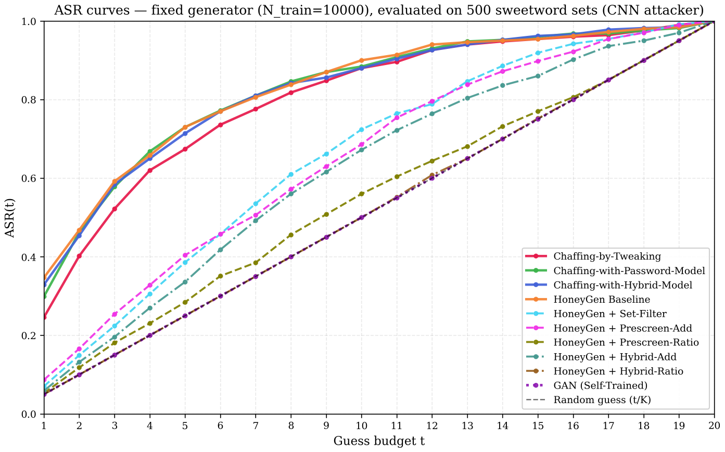
\includegraphics[width=\linewidth]{figures/cmp_N10000_e500.png}
    \caption{Test on 500 sets.}
  \end{subfigure}

  \medskip
  \begin{subfigure}{0.66\textwidth}
    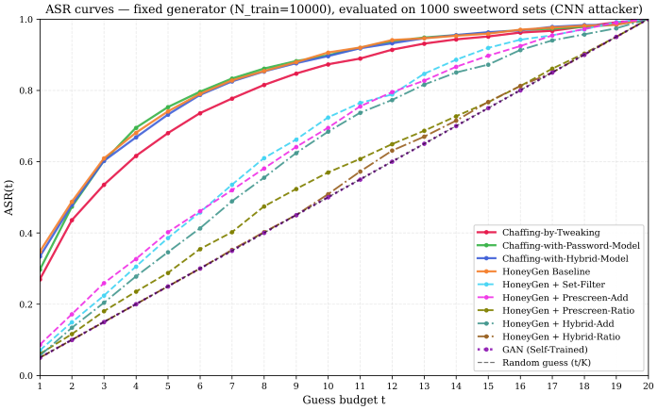
\includegraphics[width=\linewidth]{figures/cmp_N10000_e1000.png}
    \caption{Test on 1000 sets.}
  \end{subfigure}

  \medskip
  \begin{subfigure}{0.66\textwidth}
    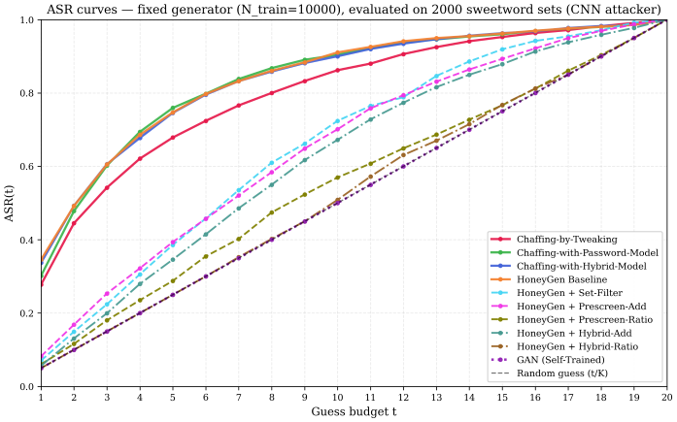
\includegraphics[width=\linewidth]{figures/cmp_N10000_e2000.png}
    \caption{Test on 2000 sets.}
  \end{subfigure}
  \caption{ASR curves under the CNN attacker at $N_{\text{train}} = 10000$
  for all ten methods, evaluated on test sets of 500, 1000, and 2000
  sweetword sets. The three panels keep the same shape and the same
  ordering of methods as the test set grows.}
  \label{fig:cmp-all}
\end{figure}

\section{The GAN Result Requires a Caveat}
\label{sec:results-gan}

% Mixed-corpus attacker figure (smaller, inline). The frequency-attacker
% results are reported in Table (tab:crossatt), not as a figure.

\begin{figure}[ht]
  \centering
  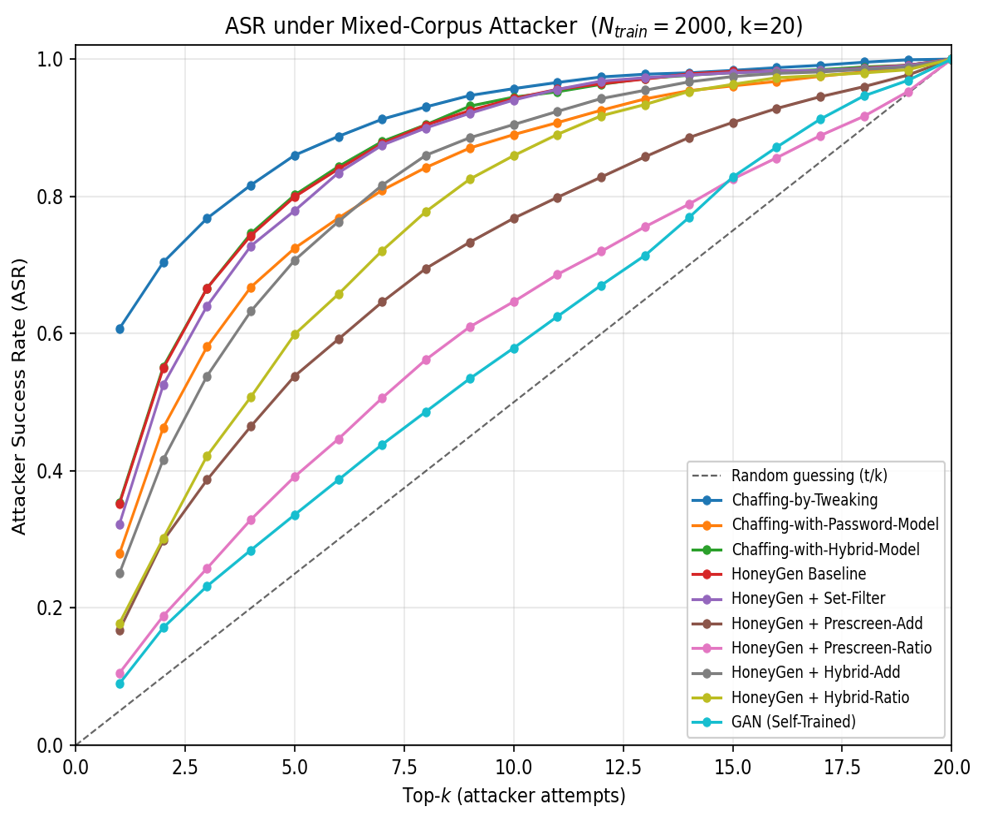
\includegraphics[width=0.72\textwidth]{figures/asr_mixed_N2000.png}
  \caption{ASR curves under the mixed-corpus attacker (trained on
  Tweak + Password-Model + HoneyGen + GAN negatives) at
  $N_{\text{train}} = 2000$, test on 2000 passwords. The GAN moves off
  the random-guessing diagonal it hugged under the single-family CNN
  attacker, and the effect strengthens with training size
  (\Cref{sec:results-gan}).}
  \label{fig:asr-mixed-2000}
\end{figure}


The GAN's reported $\mathrm{ASR}@5 = 0.872$ at $N_{\text{train}} = 10000$
(\Cref{tab:asr-master}) makes it one of the weakest methods in the
benchmark, but the reason is worth spelling out, because an attacker
that simply followed the CNN would conclude the opposite.
\Cref{tab:gan} reports two attacker strategies side by side together
with $F_{\text{rank}}$.

% ===== GAN artifact table (N_train=10000, N_eval=2000) =====
\begin{table}[t]
  \centering
  \begin{tabular}{lrrrr}
    \toprule
    \textbf{Method} & Follow-CNN & Anti-CNN & Reported & $F_{\text{rank}}$ \\
     & $\mathrm{ASR}@5$ & $\mathrm{ASR}@5$ & $\mathrm{ASR}@5$ & \\
    \midrule
    HoneyGen Baseline & 0.746 & 0.038 & 0.746 & 0.169 \\
    HoneyGen + Prescreen-Ratio & 0.341 & 0.180 & 0.341 & 0.422 \\
    HoneyGen + Hybrid-Ratio & 0.293 & 0.202 & 0.293 & 0.462 \\
    GAN (Self-Trained) & 0.025 & 0.872 & 0.872 & 0.920 \\
    \bottomrule
  \end{tabular}
  \caption{Two attacker strategies at $N_{\text{train}}=10000$:
  \emph{Follow-CNN} guesses the CNN's top-ranked candidates,
  \emph{Anti-CNN} guesses its bottom-ranked ones, and \emph{Reported}
  is the rational-attacker value of \Cref{eq:rational}. For the baseline
  and the ratio filters, Follow-CNN is the larger of the two directions
  and $F_{\text{rank}}$ sits near or above $0.4$, so the reported value
  simply follows the CNN. The GAN is the exception --- its
  $F_{\text{rank}}$ near $1$ places the real password at the bottom, so
  Follow-CNN succeeds only $2.5\%$ of the time while Anti-CNN reaches
  $87\%$. Its low Follow-CNN score is inverted distinguishability, not
  flatness.}
  \label{tab:gan}
\end{table}


For HoneyGen Baseline, following the CNN's top-ranked guesses succeeds
$74.6\%$ of the time and $F_{\text{rank}}$ is $0.169$ --- the real
password sits near the top, so the attacker just follows the CNN. For
the ratio filters both attacker directions land near the
random-guessing rate and $F_{\text{rank}}$ is close to the ideal $0.5$;
the real password is in the middle, so neither direction helps and the
sets are genuinely flat. The GAN is the exception. Following the CNN
succeeds only $2.5\%$ of the time, which taken alone would make the GAN
look like the flattest method in the benchmark, but its
$F_{\text{rank}}$ is $0.920$: the real password is ranked at or near the
bottom of almost every GAN set. A rational attacker inverts and guesses
the CNN's \emph{lowest}-scored candidates, and succeeds $87.2\%$ of the
time --- which is the value the two-sided floor of \Cref{eq:rational}
reports. A GAN trained on the oracle corpus samples from the corpus's
high-probability region, and the real password, itself a low-probability
sample, looks like an outlier the classifier confidently rejects; this
is inverted distinguishability, not flatness.

The bias is confirmed by a change of attacker. Under the
mixed-corpus attacker of \Cref{sec:method-cnn} --- trained on Tweak,
Password-Model, HoneyGen and GAN negatives together --- the GAN leaves
the random-guessing diagonal it hugged under the single-family CNN
attacker: at $N_{\text{train}} = 2000$ its $\mathrm{ASR}@5$ rises from
$0.21$ to $0.34$ (\Cref{fig:asr-mixed-2000}), and the effect grows with
training size, reaching $0.99$ at $N_{\text{train}} = 5000$, while the
filtered ratio methods shift comparatively little.
\Cref{tab:mixed} lists the per-method $\mathrm{ASR}@5$ under the two
attackers at $N_{\text{train}} = 2000$. Whether it is exposed by the
inverted CNN strategy or by a broader attacker, the GAN's apparent
flatness under a naive single-family attacker is not a property of the
sweetword sets it produces.

% ===== CNN vs Mixed attacker (N_train=2000, matches slide 15) =====
\begin{table}[t]
  \centering
  \begin{tabular}{lrr}
    \toprule
    \textbf{Method} & CNN-only $\mathrm{ASR}@5$ & Mixed-corpus $\mathrm{ASR}@5$ \\
    \midrule
    Chaffing-by-Tweaking & 0.679 & 0.860 \\
    Chaffing-with-Password-Model & 0.759 & 0.725 \\
    Chaffing-with-Hybrid-Model & 0.756 & 0.802 \\
    HoneyGen Baseline & 0.752 & 0.799 \\
    HoneyGen + Set-Filter & 0.728 & 0.779 \\
    HoneyGen + Prescreen-Add & 0.588 & 0.538 \\
    HoneyGen + Prescreen-Ratio & 0.417 & 0.392 \\
    HoneyGen + Hybrid-Add & 0.641 & 0.707 \\
    HoneyGen + Hybrid-Ratio & 0.503 & 0.599 \\
    GAN (Self-Trained) & 0.212 & 0.336 \\
    \bottomrule
  \end{tabular}
  \caption{$\mathrm{ASR}@5$ under the HoneyGen-only CNN attacker versus the
  mixed-corpus attacker (Tweak + Password-Model + HoneyGen + GAN negatives)
  at $N_{\text{train}}=2000$. The GAN moves off the near-floor value it
  reported under the CNN-only attacker ($0.21 \to 0.34$), while the
  filtered ratio methods shift comparatively little; the effect is much
  larger at $N_{\text{train}}=5000$ (\Cref{sec:results-gan}).}
  \label{tab:mixed}
\end{table}


\section{Robustness Across Attacker Class}
\label{sec:results-freq}

The filter is tuned against the CNN attacker, so we check the accepted
sets against the two robustness attackers of
\Cref{sec:method-robustness-attackers}: an independent frequency ranker
and a mixed-corpus CNN. \Cref{tab:crossatt} reports the CNN and the
frequency attacker at $N_{\text{train}} = 10000$.

% ===== Cross-attacker CNN vs Freq (N_train=10000) =====
\begin{table}[t]
  \centering
  \begin{tabular}{lrrrr}
    \toprule
    & \multicolumn{2}{c}{\textbf{CNN attacker}} & \multicolumn{2}{c}{\textbf{Freq. attacker}} \\
    \cmidrule(lr){2-3}\cmidrule(lr){4-5}
    \textbf{Method} & $\mathrm{ASR}@1$ & $\mathrm{ASR}@5$ & $\mathrm{ASR}@1$ & $\mathrm{ASR}@5$ \\
    \midrule
    Chaffing-by-Tweaking & 0.281 & 0.678 & 0.216 & 0.386 \\
    Chaffing-with-Password-Model & 0.304 & 0.755 & 0.050 & 0.250 \\
    Chaffing-with-Hybrid-Model & 0.337 & 0.743 & 0.083 & 0.319 \\
    HoneyGen Baseline & 0.346 & 0.746 & 0.084 & 0.319 \\
    HoneyGen + Set-Filter & 0.179 & 0.610 & 0.086 & 0.322 \\
    HoneyGen + Prescreen-Add & 0.144 & 0.525 & 0.050 & 0.250 \\
    HoneyGen + Prescreen-Ratio & 0.071 & 0.341 & 0.050 & 0.250 \\
    HoneyGen + Hybrid-Add & 0.141 & 0.510 & 0.068 & 0.286 \\
    HoneyGen + Hybrid-Ratio & 0.050 & 0.293 & 0.076 & 0.305 \\
        GAN (Self-Trained) & 0.745 & 0.872 & 0.225 & 0.388 \\
    \bottomrule
  \end{tabular}
  \caption{Cross-attacker comparison at $N_{\text{train}}=10000$
  (rational-attacker $\mathrm{ASR}$, \Cref{eq:rational}).
  The frequency attacker separates the methods far less sharply than the
  CNN; the filtered HoneyGen variants stay near the frequency floor. The
  GAN is distinguishable under both attackers --- most strongly by the
  CNN, which reaches $0.872$ once its ranking is inverted (the real
  password sits at the bottom), and also by the frequency attacker at
  $0.388$; it is flat under neither, as discussed in
  \Cref{sec:results-gan}.}
  \label{tab:crossatt}
\end{table}


Three points follow. First, the frequency attacker is a substantially
weaker distinguisher than the CNN: its $\mathrm{ASR}@5$ on HoneyGen
Baseline is 0.319 versus 0.746 for the CNN. This is the gap
PassFilter identified --- methods evaluated only against ranker-style
attackers report flatness numbers that overstate their security once a
learned discriminator is admitted. Second, filtering against the CNN
does not open the sets up to the frequency attacker: the filtered
variants stay near the frequency floor, so there is no security
trade-off between the two attacker classes. This absence of a trade-off
is somewhat surprising, since tuning a filter to one attacker does not
in general protect against a different one, and we do not have a proven
explanation for it. A plausible one is that the features the CNN relies
on to judge how ``real'' a candidate looks are themselves correlated
with popularity --- the common structural patterns that also drive the
frequency ranker --- so a set the CNN cannot separate tends to be one
the frequency attacker cannot separate either. We report this as an
empirical observation rather than a guarantee; whether the two attacker
classes genuinely align, or whether a trade-off appears against a
stronger ranker, is left as future work. Third, the GAN is
distinguishable to both attackers rather than flat: its frequency
$\mathrm{ASR}@5$ of 0.388 is the highest frequency value in the table,
and under the CNN a rational attacker that inverts the ranking reaches
0.872 (\Cref{sec:results-gan}). The GAN is thus caught from both
directions --- by the frequency ranker directly and by the CNN once its
anti-informative ranking is inverted.

\section{Discussion}
\label{sec:results-discussion}

The picture is consistent across training size and attacker class,
with four conclusions.

\emph{First, unfiltered honeyword generators are vulnerable to a CNN
attacker.} The four baselines report $\mathrm{ASR}@5$ around
$0.68$--$0.76$ across all three corpus sizes, about three times the
random-guessing rate, and the sophistication of the generator does not
translate into flatness.

\emph{Second, filtering restores flatness, most strongly in the ratio
variant.} The ratio filters bring $\mathrm{ASR}@5$ down to
0.341--0.293 at $N_{\text{train}} = 10000$ with $F_{\text{rank}}$
near the ideal middle, and preserve most of that reduction at smaller
sizes; the additive filters achieve a moderate reduction at a much
lower rejection cost.

\emph{Third, acceptance is a first-class requirement.} Under the
relaxed thresholds every filtered method is deployable
($>25\%$ acceptance) at every corpus size, and the recommended
configurations are the ratio filters read through the two-stage
criterion of \Cref{sec:results-cost}: the flattest methods that remain
deployable.

Fourth, the GAN's apparent success is a distributional artifact.
Following the CNN naively, the GAN looks like the flattest method, but
$F_{\text{rank}}$ far from the ideal middle value of $0.5$ ---
$0.920$, not $0$ --- shows the real password is ranked at the bottom
rather than the top, so a rational attacker who inverts the ranking
reaches $\mathrm{ASR}@5 = 0.872$ (\Cref{eq:rational}); the same bias is exposed
by the mixed-corpus attacker, and the GAN is also the most
distinguishable method under the frequency attacker. Any security claim
that treats the GAN as a strong flatness-preserving generator has to
face this data. \Cref{ch:conclusion} takes these conclusions as its
starting point.


\chapter{Conclusion}
\label{ch:conclusion}

This thesis started from a mismatch. Honeyword-based breach detection
depends on flatness --- the promise that an attacker who has read the
password file cannot identify the real credential in a sweetword set
with probability better than $1/k$ --- and every widely-deployed
honeyword generator has been evaluated against attackers that no
longer represent the state of the art. \textcite{dani2024passfilter}
showed that a small character-level CNN, trained as a binary
classifier on real-vs-decoy pairs, breaks flatness on essentially
every honeyword scheme they tested. The question this left open was
whether flatness can be restored against such an attacker without
redesigning the generator.

The answer we develop is affirmative but qualified. The same CNN
discriminator that PassFilter used as an attack,
reused unmodified as a defensive oracle at storage time, gates
sweetword sets against a small set of measurable flatness conditions.
Sets that fail are regenerated. Sets that pass are stored. The
generator itself is not modified, and neither is the attacker; only
the pipeline in which they are combined changes. On the ten-method
benchmark of \Cref{ch:results}, the two-stage filter with a
multiplicative pre-screening band reduces the attacker's $\mathrm{ASR}@5$
from around $0.75$ for the unfiltered baselines to $0.29$--$0.34$ for
the strongest configurations at $N_{\text{train}} = 10000$, with a
real password ranked near the middle of the twenty candidates
($F_{\text{rank}} \approx 0.42$--$0.46$). Under the thresholds adopted
in \Cref{sec:method-threshold-tradeoff}, these ratio filters accept
between $29\%$ and $78\%$ of passwords across corpus sizes --- well
inside the deployable range, and far above the single-digit acceptance
of the initial strict configuration.

\section{Summary of Contributions}

The concrete contributions of the thesis map to \Cref{ch:method}
and \Cref{ch:results}. First, an attacker-relative definition of
flatness formalized at the level of the attacker-induced distribution
over a sweetword set, characterized by four measurable quantities
($F_{\text{rank}}$, $F_{\text{ent}}$, top gap, and an
$\varepsilon$-flatness bound $q_{\max} \le 1/k + \varepsilon_{\max}$ on
the largest entry of the induced distribution). Second, a
hybrid flatness-filtering algorithm that combines candidate-level
pre-screening with set-level rejection sampling, generator-agnostic
and requiring no retraining of either the underlying generator or the
attacker.

The benchmark itself is the third contribution: ten honeyword
generation methods spanning rule-based tweaking,
representation-learning HoneyGen variants, and a self-trained GAN,
evaluated under a common experimental protocol at three training sizes,
and against three attacker classes --- the
HoneyGen-tuned CNN, a mixed-corpus CNN trained on several decoy
families, and a frequency ranker --- which together separate genuine
flatness from single-attacker artifacts.

\section{What the Numbers Actually Say}

Three quantitative findings deserve to be extracted from
\Cref{ch:results} and stated cleanly enough for a reader in a hurry.

Unfiltered honeyword generators are highly distinguishable to the
CNN. All four baselines (Tweaking, Password-Model, Hybrid-Model,
HoneyGen Baseline) report $\mathrm{ASR}@5$ in the range $0.68$--$0.77$
across every training-set size we tested, about three times the
random-guessing rate $0.25$.

Flatness filtering reduces $\mathrm{ASR}@5$ substantially, and the
ratio band is what does most of the work. At $N_{\text{train}} = 10000$
the Prescreen-Ratio and Hybrid-Ratio variants push $\mathrm{ASR}@5$
down to $0.341$ and $0.293$ with $F_{\text{rank}}$ near the ideal
middle value of $0.5$ --- genuine near-uniform ranking --- while the
additive filters achieve moderate reductions to the $0.51$--$0.61$
range. The relative ordering of methods is preserved as the training
corpus varies over $2000$, $5000$, and $10000$. Because acceptance is
treated as a first-class deployability requirement
(\Cref{sec:results-cost}), the recommended configurations are the
ratio filters read through a two-stage criterion: the flattest methods
among those that remain deployable.

The GAN's apparent flatness is a distributional artifact and should not
be read as a defence. Following the CNN's top guesses, its
$\mathrm{ASR}@5$ at $N_{\text{train}} = 10000$ is essentially zero, but
$F_{\text{rank}}$ is $0.920$: the real password is ranked near position
twenty on the average set. The CNN considers the GAN-generated
candidates to look \emph{more} like real passwords than the actual real
password does, so a rational attacker inverts the ranking and reaches
$\mathrm{ASR}@5 = 0.872$ --- the value the two-sided rational-attacker
floor reports, which makes the GAN one of the weakest methods in the
benchmark rather than the strongest. Two independent checks confirm the
bias rather than flatness: under the frequency attacker the same GAN
sets report $\mathrm{ASR}@5 = 0.388$, the highest in that column, and
under the mixed-corpus attacker the GAN's $\mathrm{ASR}@5$ rises from
about $0.07$ to $0.99$ at $N_{\text{train}} = 5000$. This artifact is
pronounced at the larger corpus sizes; at $N_{\text{train}} = 2000$ the
GAN's $F_{\text{rank}}$ is closer to the middle, so the inversion is a
property that sharpens as the generator is trained on more data.

\section{Limitations}
\label{sec:conclusion-limitations}

The framework has five limitations that a deployment would need to
reason about explicitly.

\paragraph{Coverage below 100\%.}
The most important limitation for real-world use is that the
countermeasure does not protect every user. The filter stores a
sweetword set only when it can certify that set as flat; when it cannot
do so within the regeneration budget, it gives up on that password, and
that account receives no flatness-guaranteed set. At the operating point
of this thesis the strongest (ratio) filters certify only between
$29\%$ and $78\%$ of passwords (\Cref{tab:accept}), which leaves a large
share of users --- in the worst case the majority --- without the
guarantee. A deployable system, however, has to protect $100\%$ of
accounts: it cannot simply refuse to store honeywords for the users it
finds difficult. As it stands the method would therefore need to be
paired with a fallback for the rejected passwords (for instance an
unfiltered set), which weakens the guarantee for exactly those users.
Reaching near-total coverage without sacrificing flatness is the single
biggest obstacle to real-world adoption, and we return to it as an open
question below.

\paragraph{Model-relative guarantees.}
The filter enforces flatness against one specific attacker: the
character-level CNN of \Cref{sec:method-cnn}. A different attacker ---
a larger CNN, a transformer, a discriminator that uses side
information beyond the password string --- may recover
distinguishability on sets the filter has certified. The guarantees
are best read as flatness against this class of learned attacker,
not as flatness in general. \Cref{sec:results-freq} shows that the
guarantees transfer partially to the frequency attacker, which is
weaker; whether they transfer to stronger models is an empirical
question that requires running each candidate attacker through the
same benchmark.

\paragraph{One-sided set-level acceptance.}
The set-level acceptance test constrains only the maximum of the
induced distribution $q$. A set in which some honeyword receives an
anomalously low $q$ would pass the test even though $q$ is not close
to uniform. In our data this does not translate into ASR degradation,
because ASR responds to the top of the ranking rather than the tail,
but the acceptance predicate could be tightened to bound both ends of
$q$. This is a small extension of \Cref{alg:hff} and would be worth
doing in a production build of the filter.

\paragraph{Acceptance-rate cost of the ratio filter.}
The strongest security in the benchmark, from the Prescreen-Ratio and
Hybrid-Ratio filters, comes at the lowest acceptance rates among the
filtered methods --- between $29\%$ and $78\%$ across corpus sizes,
against $65\%$--$97\%$ for the additive filters --- and a higher
average number of regeneration attempts, up to about $4.6$ per
accepted set (\Cref{tab:accept}). Under the relaxed thresholds this is
no longer the crippling single-digit acceptance of the initial
configuration: every filtered method clears the $25\%$ deployability
mark at every training size. The residual cost is nonetheless real and
falls entirely at storage time, since filtering happens once per
account for the lifetime of the credential. A deployment that cannot
afford the ratio filter's rejection budget can move to an additive
filter and recover most of the security gain over the unfiltered
baseline at a substantially higher acceptance rate.

\paragraph{Corpus and language.}
All experiments use the cleaned RockYou corpus, a leak of primarily
English-language, user-chosen web passwords from a specific consumer
service. The distributional properties of this corpus --- long
low-probability tails, common suffixes, digit sequences at the end
--- are what the FastText embeddings, the GAN, and the CNN all learn
to model. Whether the same numbers hold on corpora with different
structural properties (enterprise credentials, non-English leaks,
machine-generated passwords) is an empirical question. Extending the
benchmark to \emph{darkc0de} as a second corpus is on the immediate
next-steps list for this pipeline.

\section{Open Questions}

Beyond the immediate limitations, five research questions remain open.

The first is adversarial adaptation. The filter, as constructed, is a
static defense: the oracle CNN is trained once and reused. An attacker
who knew the filter existed and had access to a sample of accepted
sets could train against those sets rather than against the raw
generator output. Whether the generator, the oracle, and the attacker
can be co-trained toward a stable equilibrium at
$\mathrm{ASR}@5 \approx 0.25$ is a question this thesis does not
resolve. The pieces are in place to run the experiment; the answer
requires it.

The second is transferability across a class of attackers. The
current guarantees are against one CNN. A more useful guarantee would
be against a class of models --- for example, any CNN of bounded
depth and width, or any linear classifier over a fixed feature set.
The filter could then use an ensemble oracle that discriminates
against the worst-case member of the class.
\textcite{chakraborty2022hbat} discuss related notions in the survey,
and connecting them to the flatness formalism of
\Cref{sec:method-formalism} is a natural extension.

The third is the theoretical relationship between the flatness
metrics. $F_{\text{rank}}$, $F_{\text{ent}}$, and $\varepsilon$-flatness
are correlated but not equivalent, and the acceptance predicate uses
all three plus the top gap. It is not obvious that this is the
smallest set of conditions sufficient to bound $\mathrm{ASR}@t$, or
that all three are individually necessary. A cleaner theoretical
characterization --- an inequality connecting $q_{\text{real}}$,
$F_{\text{ent}}$, and expected $\mathrm{ASR}@t$ --- would allow the
filter to constrain fewer quantities without giving up guarantees.

The fourth is the LLM-based generator line. The construction of
\Cref{sec:method-filter} is generator-agnostic and would apply
without modification to sweetword sets produced by the
chunk-manipulation and Metropolis-Hastings large language model of
the kind reviewed in \Cref{sec:related-llm}. Whether the resulting
$\mathrm{ASR}@5$ curves match, exceed, or fall below the
ratio-filtered HoneyGen numbers reported here is an experiment worth
running.

The fifth is coverage. As the limitations above stress, the filter
protects only the passwords for which it can certify a flat set, and at
the current operating point that fraction is well below $100\%$. A
practical countermeasure must cover every account, so the open question
is how to reach near-total coverage without weakening flatness. Possible
routes include stronger or password-specific generators that produce
flat candidates more reliably, thresholds adapted per password to the
hardest cases, or a principled fallback for the residual passwords that
no generator can flatten. Which of these --- or which combination ---
closes the gap is the most important question this thesis leaves open.

\section{Closing}

Honeywords are a modest defense with an outsized property: they turn
a silent failure --- offline password recovery from a stolen hash
file --- into an observable event at the authentication server. That
property is worth preserving as attacker capabilities improve, and
the argument this thesis makes is that each new class of attacker
should be reused as an enforcement tool at storage time. The
classifier that would otherwise recover the real password becomes
the gatekeeper that prevents any sweetword set with a recoverable
real password from being stored. The reversal is small and the
numbers are moderate, but the direction feels right: as long as
attackers keep getting better, defenders can keep the same tools,
pointed the other way.


% Bibliography using biber; comment this and uncomment the following lines to use bibtex instead
\printbibliography
% \bibliographystyle{alphaurl}
% \bibliography{bib}

\end{document}

